% Options for packages loaded elsewhere
\PassOptionsToPackage{unicode}{hyperref}
\PassOptionsToPackage{hyphens}{url}
%
\documentclass[
]{article}
\usepackage{amsmath,amssymb}
\usepackage{lmodern}
\usepackage{iftex}
\ifPDFTeX
  \usepackage[T1]{fontenc}
  \usepackage[utf8]{inputenc}
  \usepackage{textcomp} % provide euro and other symbols
\else % if luatex or xetex
  \usepackage{unicode-math}
  \defaultfontfeatures{Scale=MatchLowercase}
  \defaultfontfeatures[\rmfamily]{Ligatures=TeX,Scale=1}
\fi
% Use upquote if available, for straight quotes in verbatim environments
\IfFileExists{upquote.sty}{\usepackage{upquote}}{}
\IfFileExists{microtype.sty}{% use microtype if available
  \usepackage[]{microtype}
  \UseMicrotypeSet[protrusion]{basicmath} % disable protrusion for tt fonts
}{}
\makeatletter
\@ifundefined{KOMAClassName}{% if non-KOMA class
  \IfFileExists{parskip.sty}{%
    \usepackage{parskip}
  }{% else
    \setlength{\parindent}{0pt}
    \setlength{\parskip}{6pt plus 2pt minus 1pt}}
}{% if KOMA class
  \KOMAoptions{parskip=half}}
\makeatother
\usepackage{xcolor}
\usepackage[margin=1in]{geometry}
\usepackage{longtable,booktabs,array}
\usepackage{calc} % for calculating minipage widths
% Correct order of tables after \paragraph or \subparagraph
\usepackage{etoolbox}
\makeatletter
\patchcmd\longtable{\par}{\if@noskipsec\mbox{}\fi\par}{}{}
\makeatother
% Allow footnotes in longtable head/foot
\IfFileExists{footnotehyper.sty}{\usepackage{footnotehyper}}{\usepackage{footnote}}
\makesavenoteenv{longtable}
\usepackage{graphicx}
\makeatletter
\def\maxwidth{\ifdim\Gin@nat@width>\linewidth\linewidth\else\Gin@nat@width\fi}
\def\maxheight{\ifdim\Gin@nat@height>\textheight\textheight\else\Gin@nat@height\fi}
\makeatother
% Scale images if necessary, so that they will not overflow the page
% margins by default, and it is still possible to overwrite the defaults
% using explicit options in \includegraphics[width, height, ...]{}
\setkeys{Gin}{width=\maxwidth,height=\maxheight,keepaspectratio}
% Set default figure placement to htbp
\makeatletter
\def\fps@figure{htbp}
\makeatother
\setlength{\emergencystretch}{3em} % prevent overfull lines
\providecommand{\tightlist}{%
  \setlength{\itemsep}{0pt}\setlength{\parskip}{0pt}}
\setcounter{secnumdepth}{5}
\newlength{\cslhangindent}
\setlength{\cslhangindent}{1.5em}
\newlength{\csllabelwidth}
\setlength{\csllabelwidth}{3em}
\newlength{\cslentryspacingunit} % times entry-spacing
\setlength{\cslentryspacingunit}{\parskip}
\newenvironment{CSLReferences}[2] % #1 hanging-ident, #2 entry spacing
 {% don't indent paragraphs
  \setlength{\parindent}{0pt}
  % turn on hanging indent if param 1 is 1
  \ifodd #1
  \let\oldpar\par
  \def\par{\hangindent=\cslhangindent\oldpar}
  \fi
  % set entry spacing
  \setlength{\parskip}{#2\cslentryspacingunit}
 }%
 {}
\usepackage{calc}
\newcommand{\CSLBlock}[1]{#1\hfill\break}
\newcommand{\CSLLeftMargin}[1]{\parbox[t]{\csllabelwidth}{#1}}
\newcommand{\CSLRightInline}[1]{\parbox[t]{\linewidth - \csllabelwidth}{#1}\break}
\newcommand{\CSLIndent}[1]{\hspace{\cslhangindent}#1}
\usepackage{float} \floatplacement{figure}{H} \newcommand{\beginsupplement}{\setcounter{table}{0}  \renewcommand{\thetable}{S\arabic{table}} \setcounter{figure}{0} \renewcommand{\thefigure}{S\arabic{figure}}} \usepackage{caption} \captionsetup[figure]{font=small} \usepackage{fancyhdr} \pagestyle{fancy}
\ifLuaTeX
  \usepackage{selnolig}  % disable illegal ligatures
\fi
\IfFileExists{bookmark.sty}{\usepackage{bookmark}}{\usepackage{hyperref}}
\IfFileExists{xurl.sty}{\usepackage{xurl}}{} % add URL line breaks if available
\urlstyle{same} % disable monospaced font for URLs
\hypersetup{
  hidelinks,
  pdfcreator={LaTeX via pandoc}}

\title{Object image size is a fundamental coding dimension\\
in human vision: new insights and model}
\author{Tim S. Meese \& Daniel H. Baker (2023)\\
\emph{Neuroscience}, \textbf{413}: 79-91\\
DOI: \href{https://dx.doi.org/10.1016/j.neuroscience.2023.01.025}{10.1016/j.neuroscience.2023.01.025}}
\date{}

\begin{document}
\maketitle

\fancyhead[RE,RO]{Meese \& Baker (2023), Neuroscience, 413: 79-91. DOI: 10.1016/j.neuroscience.2023.01.025}

\hypertarget{abstract}{%
\section*{Abstract}\label{abstract}}
\addcontentsline{toc}{section}{Abstract}

In previous psychophysical work we found that luminance contrast is integrated over retinal area subject to contrast gain control. If different mechanisms perform this operation for a range of superimposed retinal regions of different sizes, this could provide the basis for size-coding. To test this idea we included two novel features in a standard adaptation paradigm to discount more pedestrian accounts of repulsive size-aftereffects. First, we used spatially jittering luminance-contrast adaptors to avoid simple contour displacement aftereffects. Second, we decoupled adaptor and target spatial frequency to avoid the well-known spatial frequency shift aftereffect. Empirical results indicated strong evidence of a bidirectional size adaptation aftereffect. We show that the textbook population model is inappropriate for our results, and develop our existing model of contrast perception to include multiple size mechanisms with divisive surround-suppression from the largest mechanism. For a given stimulus patch, this delivers a blurred step-function of responses across the population, with contrast and size encoded by the height and lateral position of the step. Unlike for textbook population coding schemes, our human results (\emph{N}=4 male, \emph{N}=4 female) displayed two asymmetries: (i) size aftereffects were greatest for targets smaller than the adaptor, and (ii) on that side of the function, results did not return to baseline, even when targets were 25\% of adaptor diameter. Our results and emergent model properties provide evidence for a novel dimension of visual coding (size) and a novel strategy for that coding, consistent with previous results on contrast detection and discrimination for various stimulus sizes.

\textbf{Keywords}: adaptation; size perception; gain control; visual psychophysics; computational model

\hypertarget{introduction}{%
\section*{Introduction}\label{introduction}}
\addcontentsline{toc}{section}{Introduction}

A common view of early vision is that it performs local analyses of the retinal image to encode basic image features. Physiological evidence points to cells in early visual areas with appropriate selectivity, and psychophysical adaptation aftereffects suggest a population basis for the coding. This includes, motion (Mather et al., 2008; Sutherland, 1961), colour (Webster and Leonard, 2008), orientation (Coltheart, 1971; Gibson and Radner, 1937), spatial frequency (Blakemore and Sutton, 1969), binocular disparity (Blakemore and Julesz, 1971; Tsai and Victor, 2003) and duration (Heron et al., 2012; Walker et al., 1981). Adaptation aftereffects are also found in other sensory domains including those for pitch (Christman, 1954), loudness (Marks, 1994), temperature (Arnold et al., 1982), odour (Lawless, 1991) and audio-visual timing (Roach et al., 2011).

These perceptual phenomena have been used to develop our understanding of the sensory coding dimensions used by the human brain, but one obvious candidate missing from the list above is that of size. There are probably several reasons for this. First, retinal image size is often lumped in with retinal spatial frequency (e.g. Webster and Leonard, 2008) but as we shall show, these are two separate adaptable stimulus dimensions with different underlying mechanisms. Second, there is a view that size mechanisms have already been identified psychophysically by using adapt and test stimuli with different diameters, for example. However, as we review in this discussion, results from those studies might derive from perceptual contour displacement, not size-mechanisms per se. Finally, there is a view that the problem of retinal image size and position is solved in the primary visual cortex because it is retinotopically mapped. While local signs might at least be involved in the encoding of relative position on the retina (Morgan et al., 1990), it is no more suitable as a route for encoding size as it is for orientation, a feature for which dedicated orientation-tuned mechanisms are well-known and celebrated.

\begin{figure}

{\centering 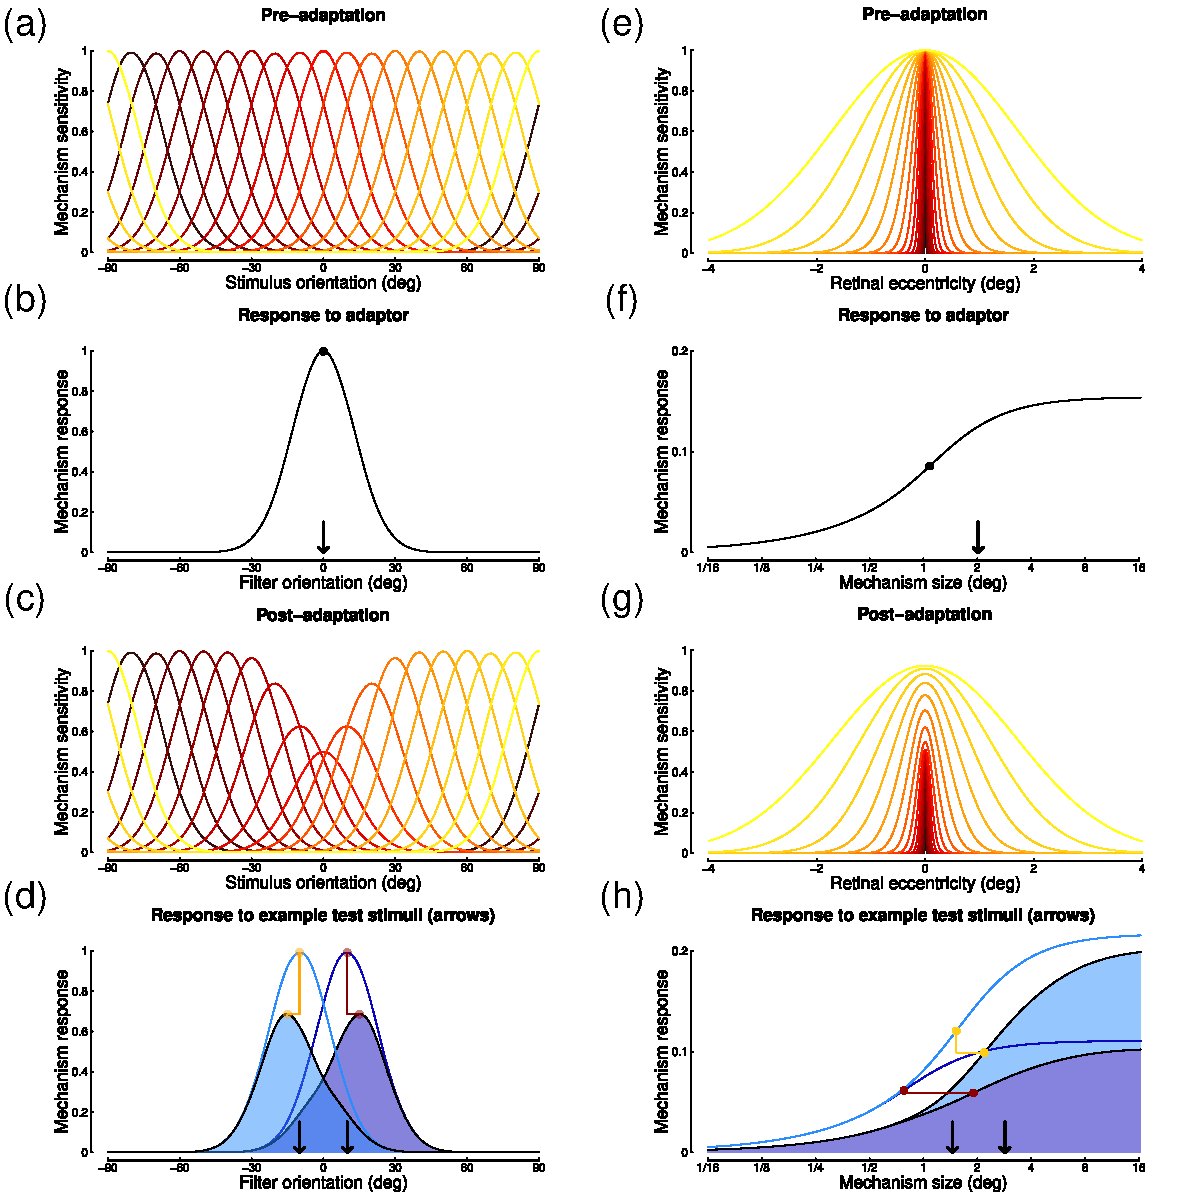
\includegraphics[width=0.8\linewidth]{Figures/Figure1} 

}

\caption{The standard ‘textbook’ model for orientation-coding and adaptation (the tilt aftereffect) (a-d) applied to size-coding and adaptation (e-h). A bank of orientation-tuned spatial filters (a) responds selectively (b) to stimulus orientation (black arrow) encoded by the peak of the response distribution. Following adaptation at this orientation, the sensitivities of nearby mechanisms are attenuated in proportion to their response to the adaptor (c), distorting the population codes (d) for nearby stimuli (black arrows) and resulting in a repulsive tilt aftereffect. (In (d) the thin curves show the response distributions for two stimuli (black arrows) pre-adaptation, and the filled curves are for those same stimuli post-adaptation.) For a population of size mechanisms, the arrangement of mechanism sensitivities along the coding dimension is different (e) from the orientation case (a). The population response to a stimulus of a given size (e.g. an adaptor; black arrow) resembles a blurred step-edge (f). For this situation the population code is not summarised by the location of its peak, as in (b), but its gradient maximum (black dot). (This happens to be to the left of the nominal stimulus size (black arrow), but this is unimportant for our purposes here). This blurred step-edge distribution means that adaptation desensitises all of the mechanisms smaller than the adapter and, to a lesser extent, some of those that are larger (g). It follows that this model predicts that adaptation will increase the perceived size of stimuli both larger and smaller than the adaptor (note the rightward shifts in gradient maxima (dots) in panel h)—i.e. it is not generally repulsive. The purpose of (e-h) is to illustrate the details of a basic size adaptation model, but thus is not the model we advocate. See text for further details, including the problems involved in trying to achieve an arrangement like that in (a-d) for size.}\label{fig:figure1}
\end{figure}

On the face of it, one might suppose that the size of a patch of grating, for example, could be encoded by a population of size-selective mechanisms along the lines of the standard population model. Figure \ref{fig:figure1}a-d shows the textbook idea for orientation coding and the tilt aftereffect (see caption for details). A similar arrangement can be envisaged for spatial frequency. Note that the narrow tuning of the mechanisms derives from the difference of Gaussian-type arrangement of the underlying receptive fields (i.e.~elongated excitatory centres for luminance with subtractive inhibition from flanking surrounds; not shown).

Modelers of size-adaptation might proceed by simply relabeling the orientation axes in Figures \ref{fig:figure1}a-d.~However, this would leave the problem of how to get from retinal image size to a standard population code with the appropriate characteristics. For orientation and spatial frequency, this is straightforward, but the situation is not so simple for retinal image size. Figure \ref{fig:figure1}e shows that (unlike for orientation and spatial frequency), a population of mechanisms that integrate luminance contrast over area (Meese and Summers, 2012; Richard et al., 2019) do not sample the coding dimension at regular intervals, but with considerable overlap and a common centre, which means the population response for a given stimulus is not the familiar bell-shaped curve (Figure \ref{fig:figure1}b), but a blurred step-edge (Figure \ref{fig:figure1}f), where the rising region owes to the benefit of contrast integration within mechanism. The arrangement might be revised by supposing difference of Gaussian-type second-order mechanisms with contrast integration windows of various sizes and inhibitory contributions from contrast in the surrounds. However, this is not the remedy it might seem. First, while the arrangement benefits mechanism selectivity, in that small mechanisms are quashed by large stimuli, it fails the other way around, in that small stimuli will excite equally all the mechanisms that are greater than or equal to the stimulus size. A fix for this is to normalise each mechanism's sensitivity by its integration area, but that arrangement kills the benefit of stimulus area at detection threshold for which evidence shows a signal integration process (Meese, 2010; Meese and Summers, 2012, 2009). Second, surround suppression from outside the classical receptive field is not subtractive, but divisive. This is true for cortical cells (Cavanaugh et al., 2002) and for the mechanisms derived from visual psychophysics (Foley, 1994; Meese, 2004; Snowden and Hammett, 1998) and is inconsistent with the assumptions underlying the standard model. Third, regardless of the arrangement for suppression, these mechanisms will confound an increase in stimulus contrast area (within the excitatory part of its mechanisms) with an increase in image contrast. Similarly, as stimulus size increases, larger mechanisms will respond more strongly than the smaller mechanisms did for the same level of contrast (e.g.~compare the two solid pre-adapt curves in Figure \ref{fig:figure1}h). This model feature is consistent with contrast detection thresholds (Meese and Summers, 2012) but not with the perception and discrimination of suprathreshold contrast (Cannon and Fullenkamp, 1988; Meese et al., 2005) and is all very different from the population behaviour of the standard model (Figures \ref{fig:figure1}a-d). Of course, one might appeal to the process of contrast gain control (as we have done elsewhere and will do here) but this raises questions about the method of implementation and still leaves the problem of how to extract an estimate of stimulus properties from the population code which is not as simple as it is for the tidier standard model (see Figure \ref{fig:figure1}). We suggest that the first derivative of the response distribution (Figures \ref{fig:figure1}f, h) is a useful approach, and return to this in a later section.

With the above in mind, our motives were two-fold. First, we wanted to know whether we could find evidence for size mechanisms in human vision. Second, should they be evidenced by repulsive adaptation aftereffects, the standard population model would need considerable development for it to provide a plausible account of this result while remaining consistent with contrast perception. However, we were far from daunted. Our previous work on the detection and discrimination of luminance contrast provided evidence for the spatial integration of contrast signals across the retinal image, a sound starting point for the construction of size mechanisms. This contrast integration was found in both the excitatory and suppressive pathways of a contrast gain control network (Baker et al., 2013); Meese and Baker, 2013; Meese and Baker, 2011; Meese and Summers, 2012; Meese and Summers, 2007). For example, by manipulating both stimulus size and extrinsic uncertainty, Meese and Summers (2012) rejected contemporary (signal detection theory) accounts of probability summation for area summation of grating contrast at detection threshold. Instead, those results provided evidence for a process that sums (exponentiated) contrast and internal noise over contiguous regions of the retina. Other experiments using novel spatial stimulus designs tailored to the issue came to the same conclusion (Baldwin and Meese, 2015; Meese, 2010; Meese and Baker, 2011; Meese and Summers, 2009; Meese and Summers, 2007). Furthermore, strong evidence for this spatial integration of contrast was found when the enquiry was extended above threshold using pedestal masking (Meese and Baker, 2011; Meese and Summers, 2007) and contrast matching (Meese et al., 2017). Crucially, in those experiments, the suprathreshold integration process was seen only with help of `Battenberg' or `Swiss cheese' stimuli (essentially, these are gratings containing evenly spaced holes) because under normal circumstances, when the area of both target and pedestal increase together, the benefit of signal integration is hidden by a concomitant process of suppression. This provides the solution to one of the problems outlined above: the visual system does not confound stimulus area with contrast because of the opposing operations of spatial integration and spatial suppression. These findings prompted a cartoon model involving a population of size-mechanisms each subject to suppressive gain control from the largest spatial region in the pool (Meese and Baker, 2011). From this, we developed the hypothesis that spatial pooling of luminance contrast might provide the basis of a population code for retinal image size in visual cortex (Meese and Baker, 2011) (e.g.~for a patch of grating), and that adapting this population would distort the perception of stimulus size.

To test this prediction, we conducted a series of novel adaptation experiments designed to isolate the putative size-coding mechanisms predicted by our hypothesis. The outcome is supported by our formalisation of a computational model developed from the earlier work on contrast perception referred to above, where surprising asymmetric features in our size-adaptation data are emergent properties of the model.

\hypertarget{experimental-procedures}{%
\section*{Experimental Procedures}\label{experimental-procedures}}
\addcontentsline{toc}{section}{Experimental Procedures}

\hypertarget{participants}{%
\subsection*{Participants}\label{participants}}
\addcontentsline{toc}{subsection}{Participants}

Participants were eight undergraduate students in their early twenties, who participated for course credit. They had no known visual abnormalities and gave written informed consent. The second author also served as a participant in a follow-up experiment. Any prescribed optical correction typically used for near work was also worn during testing. The work was conducted with the ethical approval of Aston's School of Life and Health Sciences (now the College of Health and Life Sciences).

\hypertarget{equipment}{%
\subsection*{Equipment}\label{equipment}}
\addcontentsline{toc}{subsection}{Equipment}

Stimuli were displayed on a Phillips MGD403 19-inch greyscale monitor, running at a resolution of 1280 \(\times\) 1025 pixels, with a refresh rate of 80Hz. The mean luminance of the monitor was 150\(cd/m^2\). The monitor was viewed from 103cm, at which one degree of visual angle subtended 64 pixels on the display. Participants placed their heads in a head-and-chin rest positioned at the appropriate distance and were instructed to fixate on a central cross throughout. We generated stimuli using Matlab and rendered them using a VSG2/5 framestore device (Cambridge Research Systems Ltd., Kent, UK). Participants made responses using a Kensington Expert Mouse Pro trackball device -- this is a stationary device housing a ball that could be rotated to provide dynamic adjustment of the stimulus on the screen.

\hypertarget{stimuli}{%
\subsection*{Stimuli}\label{stimuli}}
\addcontentsline{toc}{subsection}{Stimuli}

Stimuli were sinusoidal gratings, windowed by a raised cosine envelope with a blur width of 4 pixels added to each side of the plateau of the envelope. (The width of the plateau was the nominal width of the stimulus). All stimuli had a Michelson contrast of 50\%. Target stimuli were always horizontal, whereas adapting stimuli were either horizontal or vertical depending on the experiment. In experiments where size was manipulated, all stimuli had a spatial frequency of 4c/deg, and adaptors and targets varied in size (adaptors either 1 or 2 degrees, and targets from 0.25 to 8 degrees at seven levels in proportion to the adaptor; see Figure \ref{fig:figure3}a for examples). In experiments where spatial frequency was manipulated, target stimuli were the same size as the adaptor (either 1 or 2 degrees) but varied in spatial frequency between 1 and 16 c/deg (see Figure \ref{fig:figure3}b for examples).

\hypertarget{procedure}{%
\subsection*{Procedure}\label{procedure}}
\addcontentsline{toc}{subsection}{Procedure}

Figure \ref{fig:figure2} outlines the main procedure. Trials were blocked by adaptation condition throughout. The adaptor was presented to the left of a central fixation cross for 60 seconds at the start of a block (initial adaptation), and 10 seconds before each trial (top-up adaptation). The adaptor was always a sinusoidal grating with a spatial frequency of 4c/deg and a diameter of either 1 degree (4 cycles) or 2 degrees (8 cycles). During adaptation, the adaptor moved to a random spatial position every 250 ms, with the range of possible positions constrained to lie within the boundary of an invisible circle with a diameter of 4 degrees (for the small adaptor) or 8 degrees (for the large adaptor; see upper panel of Figure \ref{fig:figure2}). After adaptor offset, there was a blank period of 500 ms, followed by a target presentation of 250 ms, accompanied by a beep. The target was offset to the left of fixation by 2.5 degrees (for conditions with a 1 degree adaptor), or 5 degrees (for conditions with a 2 degree adaptor). The target then disappeared, and a matching stimulus was presented to the right of the fixation cross, offset by the same distance. In some blocks this was a thin grey ring, the diameter of which was adjusted by moving the trackball. In the remaining blocks it was another sine-wave grating, and moving the trackball adjusted the spatial frequency. The starting size or spatial frequency of the match had equal probability of being larger or smaller (or lower or higher in frequency) than the target. Once the participant was satisfied with their judgement, they clicked a button on the trackball to initiate the next trial.

\begin{figure}

{\centering 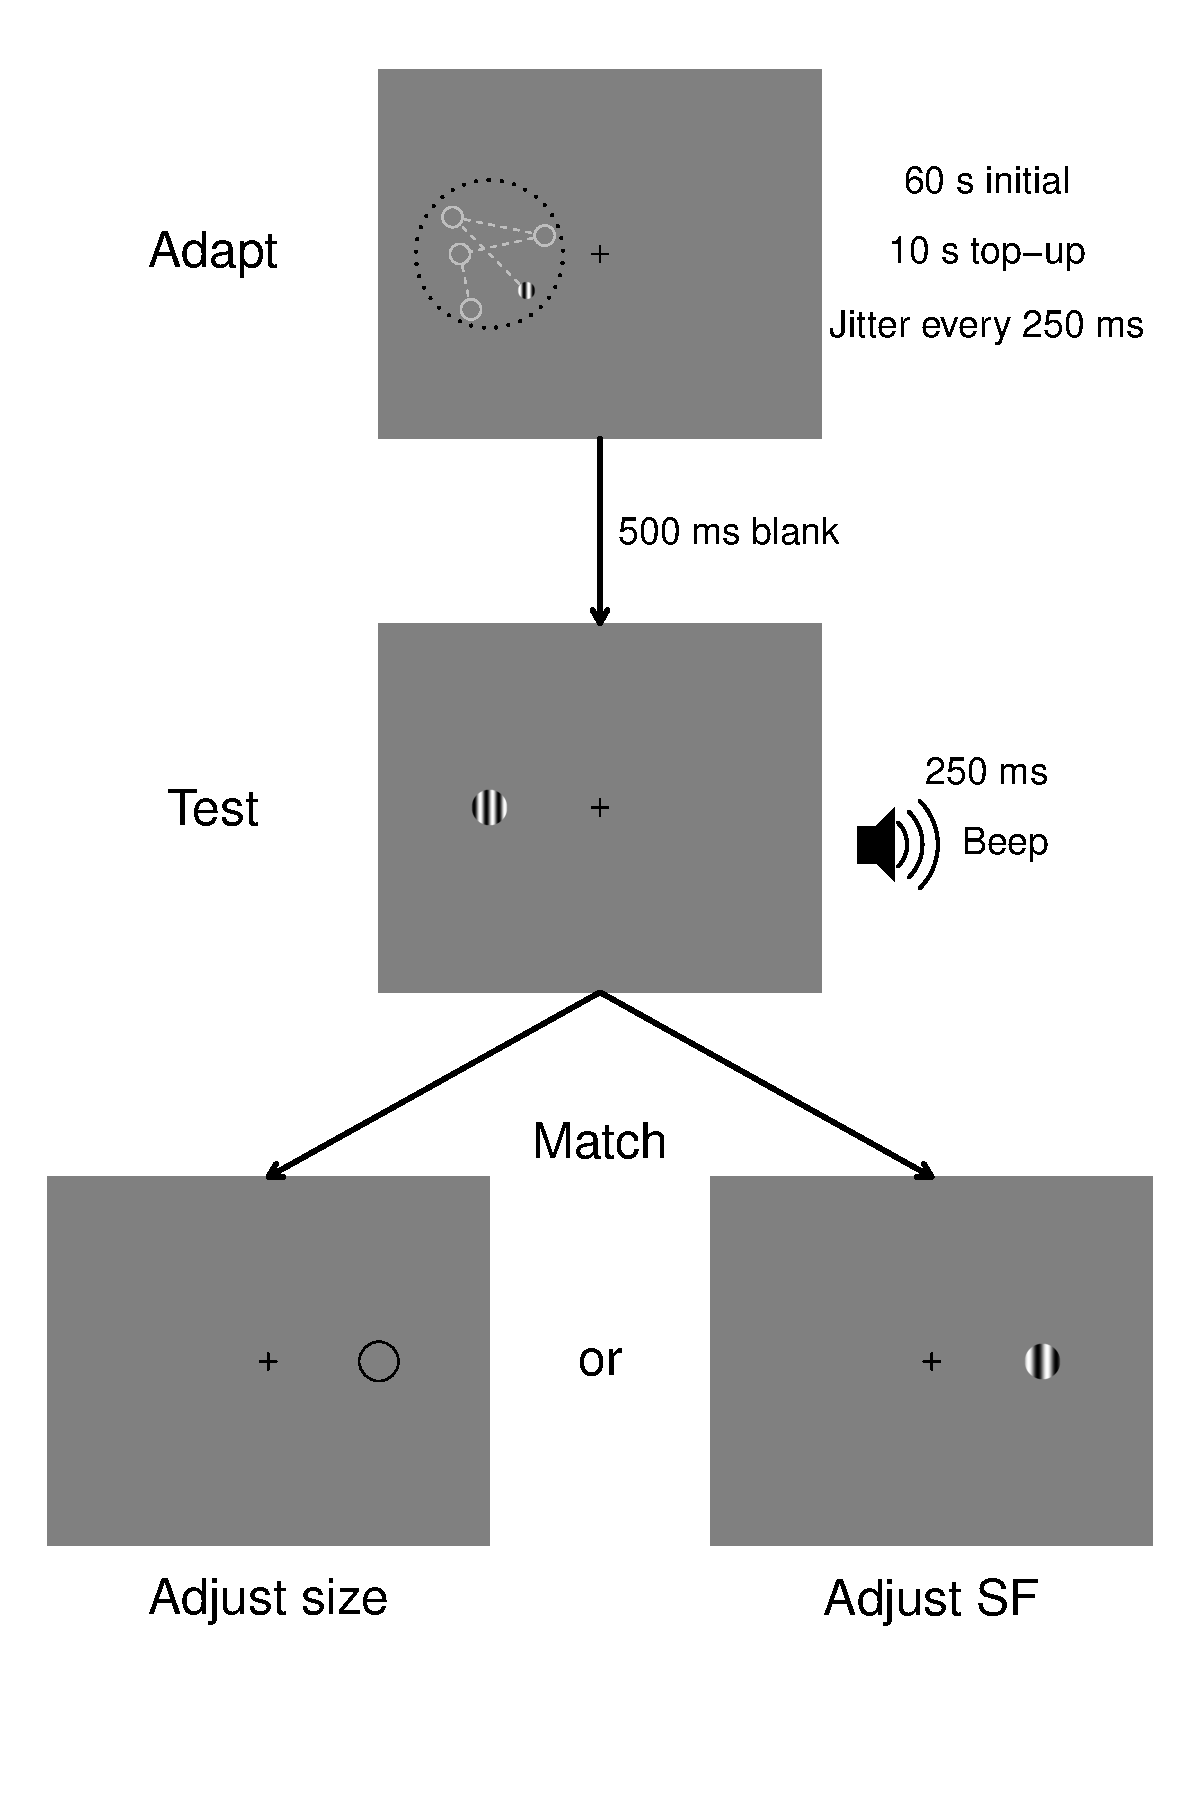
\includegraphics[width=0.5\linewidth]{Figures/Figure2} 

}

\caption{Schematic illustration of the stimulus arrangement and adaptation regime. Adapting stimuli (top panel) moved to random spatial positions to the left of a central fixation cross (the dotted circle shows the region covered by the adaptors) for a 60 second adaptation period at the start of each block of trials, and a 10 second top-up period between trials. The target stimulus was then presented to the left of fixation for 250 ms, indicated by a beep (middle panel). In different experiments, participants adjusted either the diameter of a black ring or the spatial frequency of a grating patch, both shown to the right of fixation in the unadapted region of the visual field, until it matched their perception of the target.}\label{fig:figure2}
\end{figure}

Baseline conditions were as described above, except that there was no adaptation sequence. We collected baseline data for each session before any adaptation took place, and each participant adapted to only one orientation on a given day. For conditions in the main experiment where the target size varied and spatial frequency was judged, the matching stimulus always had the same diameter as the target. In the control experiment, the matching stimulus had a fixed diameter of either 1 or 2 degrees. Each target condition (target size or spatial frequency) was repeated four times in each block, and each adaptation condition was repeated twice by each participant. Overall, participants completed 1,344 settings each across 168 distinct conditions (7 target levels \(\times\) 2 adaptor types \(\times\) 2 adaptation conditions \(\times\) 6 sub-experiments) in the main experiment, and a further 112 settings each across 14 conditions (7 target sizes \(\times\) 2 match sizes) in the control experiment.

\hypertarget{quantification-and-statistical-analysis}{%
\subsection*{Quantification and statistical analysis}\label{quantification-and-statistical-analysis}}
\addcontentsline{toc}{subsection}{Quantification and statistical analysis}

All analyses were conducted in R. The mean setting (in log units) for each participant and condition was calculated across all 8 repetitions. We calculated the percentage shift in perceived size (or spatial frequency) relative to the baseline settings. The mean and standard error of this adaptation effect were then calculated across participants. We performed a frequentist 2 (adaptor size) by 7 (target size or spatial frequency) repeated measures ANOVA for each experiment using the log values. All degrees of freedom were Greenhouse-Geisser corrected where Mauchly's test of sphericity was significant, and we report generalised eta-squared as a measure of effect size (Olejnik and Algina, 2003). We also conducted a Bayesian ANOVA (Rouder et al., 2012) (using the BayesFactor R package), allowing us to report Bayes factor scores corresponding to the main effects and interactions.

\hypertarget{data-and-software-availability}{%
\subsection*{Data and software availability}\label{data-and-software-availability}}
\addcontentsline{toc}{subsection}{Data and software availability}

Experimental scripts, raw data, analysis scripts and modelling code are available at: \url{https://osf.io/kthg3/} (DOI: 10.17605/OSF.IO/KTHG3)

\hypertarget{results}{%
\section*{Results}\label{results}}
\addcontentsline{toc}{section}{Results}

\emph{Main Experiments: Manipulations of size, spatial frequency and orientation}

Human participants (\emph{N}=8) were presented with an adapting stimulus (a patch of sine wave grating) on the left side of a computer monitor, which jittered in position (Baker and Meese, 2012; Storrs and Arnold, 2017) every 250ms to avoid causing retinal afterimages (Köhler and Wallach, 1944). They were then shown a target stimulus in the adapted region of the display and asked to report its perceived size by adjusting the diameter of a ring on the opposite side of the display (see Figure \ref{fig:figure2}). Compared to unadapted baselines (which were approximately veridical as summarised in Supplementary Figure S1), when the target was smaller than the adaptor, its perceived size reduced by around 20\%. When the target was larger than the adaptor, its perceived size increased by around 10\% (see Figure \ref{fig:figure3}a). These effects were consistent across two different sizes of adaptor and are robust and compelling in demonstrations (see Supplementary Movie S1). A factorial (7 stimulus size \(\times\) 2 adaptor size) repeated measures ANOVA indicated that the main effect of relative stimulus size was significant (F(2.3,16.3) = 18.64, p \textless0.001, \(\eta^2_g\) = 0.54, \(log_{10}BF_{10}\) = 15.1), but there was no effect of absolute adaptor size (F(1,7) = 0.005, p = 0.95, \(\eta^2_g\) \textless0.01, \(log_{10}BF_{10}\) = -0.7), nor any interaction (F(6,42) = 1.44, p = 0.22, \(\eta^2_g\) = 0.04, \(log_{10}BF_{10}\) = -0.8).

\begin{figure}
\centering
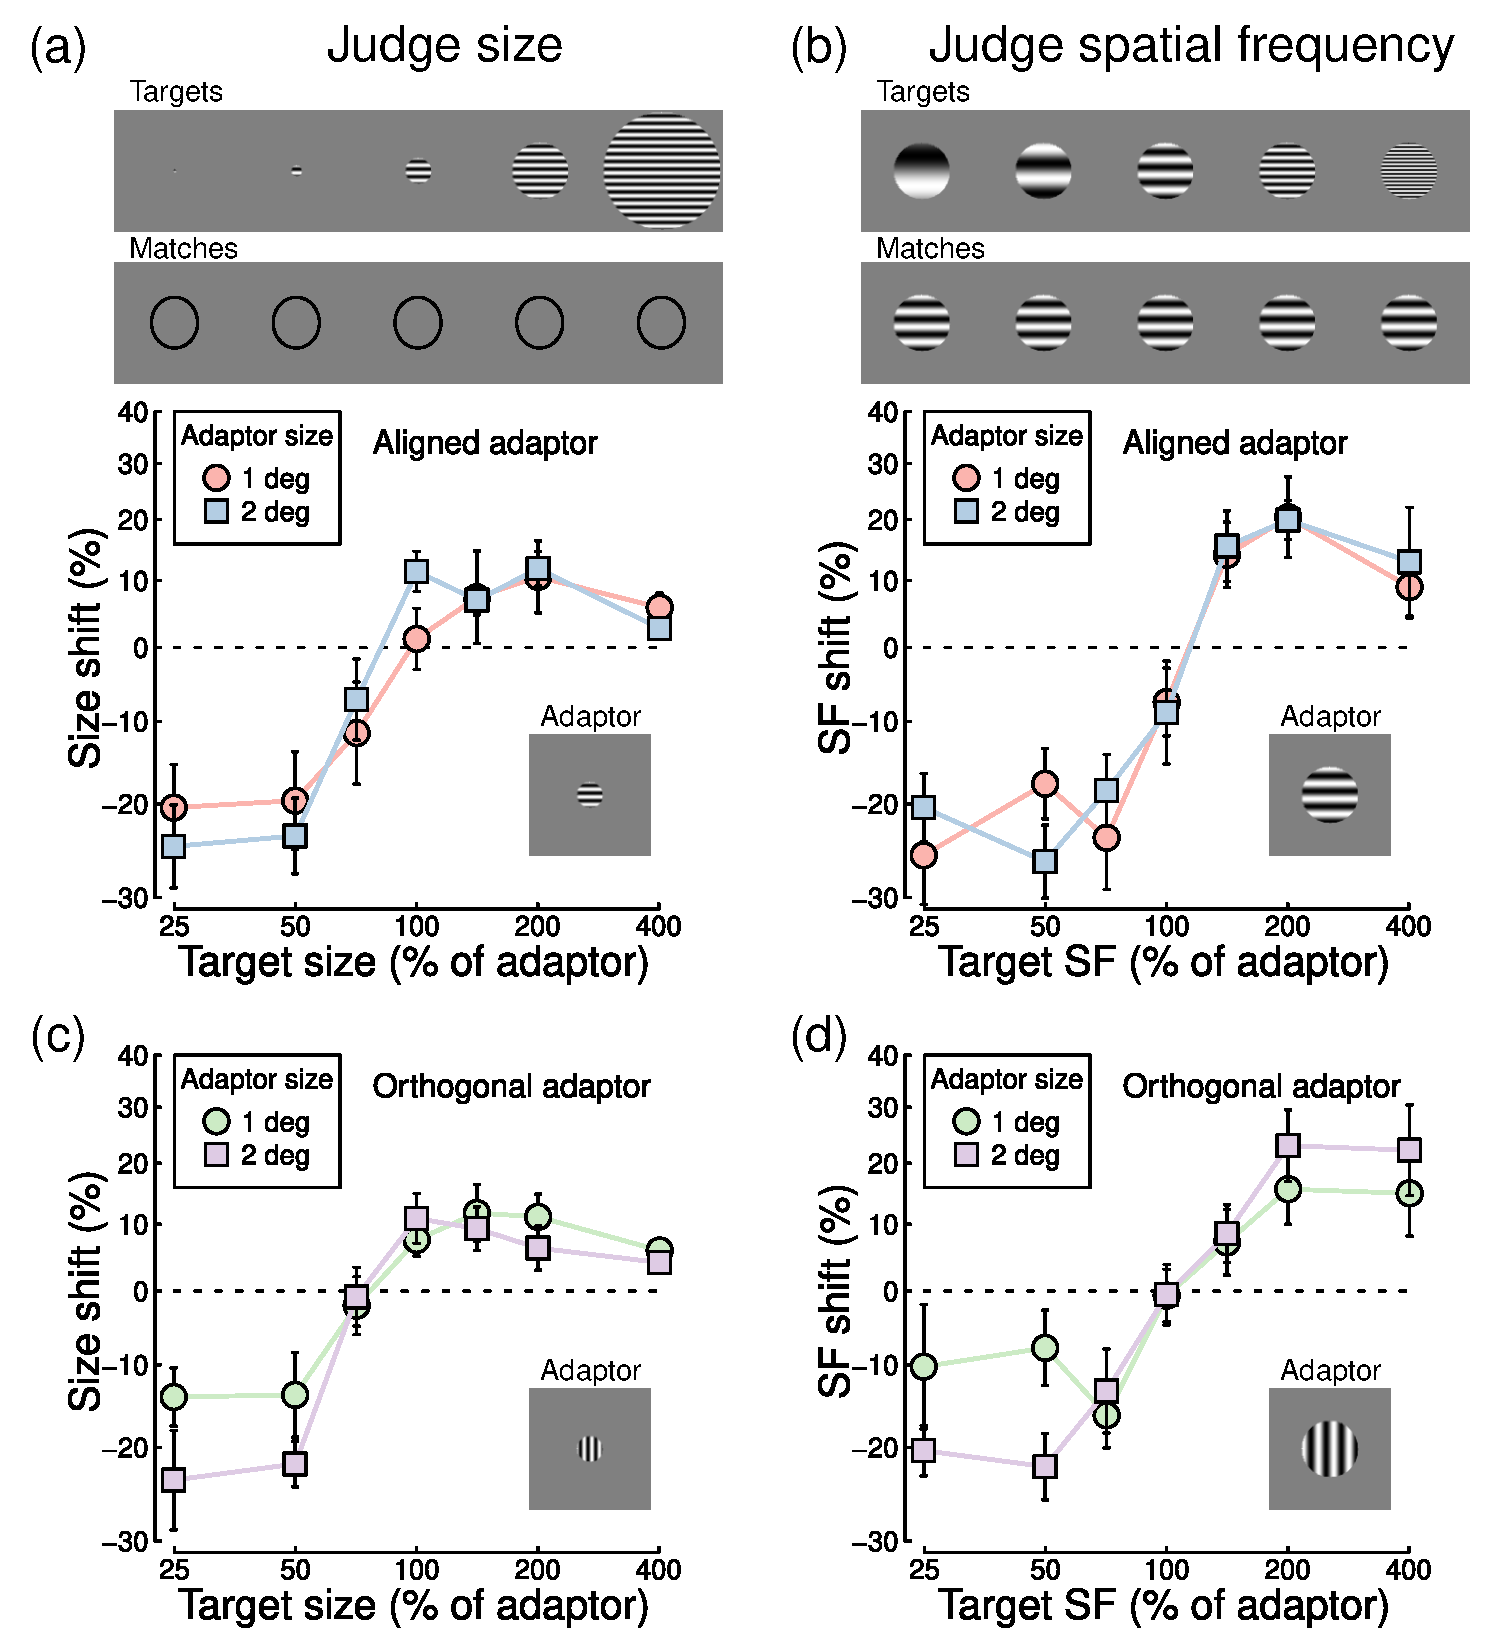
\includegraphics{Figures/Figure3.pdf}
\caption{\label{fig:figure3}Adaptation aftereffects for four experiments (\(N\) = 8 participants). The stimulus icons (top row) depict examples of the target stimuli relating to the x-axes. (They are for the 1 and 2 deg adaptor conditions on the left and right, respectively, where the adaptors are shown by the lower right inset patches.) Panel (a) shows the percentage change in perceived size as a function of target size, expressed relative to the size of the adaptor. Data are shown for two adaptor sizes (different symbols). The spatial frequency was 4 c/deg. For the 2 deg adaptor, the targets had twice the diameter shown by the icons. Panel (b) shows adaptation aftereffects for perceived spatial frequency (SF). Adaptors, targets and matches were the same size. Panels (c) and (d) show results for orthogonal orientations between target and adaptor. All panels show results relative to baseline measures where there was no adaptation (see Supplementary Figure S1). Error bars in all panels indicate ±1SE across participants (\(N\)=8), and horizontal dashed lines show baselines in the absence of adaptation.}
\end{figure}

We then sought to replicate a classic aftereffect in which the coarseness of the texture (but not the size of the patch) is affected by adaptation (Blakemore and Sutton, 1969) using our jittering adaptor (see Supplementary Movie S2). The method remained the same but this time the targets had a constant size and varied in spatial frequency (i.e.~bar width). The perceived target spatial frequency was indicated by adjusting the spatial frequency of a matching patch of grating on the opposite side of the display. This experiment also produced a repulsive aftereffect of around 20\% in each direction (see Figure \ref{fig:figure3}b; note the logarithmic y-axis). The effect of target spatial frequency was significant (F(6,42) = 24.74, p = \textless0.001, \(\eta^2_g\) = 0.599, \(log_{10}BF_{10}\) = 15.88), but there was no effect of adaptor size (F(1,7) = 0.05, p = 0.823, \(\eta^2_g\) = 0.001, \(log_{10}BF_{10}\) = -0.7), nor any interaction (F(6,42) = 0.59, p = 0.738, \(\eta^2_g\) = 0.035, \(log_{10}BF_{10}\) = -0.88). Note that spatial frequency-specific aftereffects of this kind were originally referred to as `size adaptation' (Blakemore and Sutton, 1969) and understood in terms of a population code for spatial frequency. In principle, this scheme can explain the distorting effects (Altan and Boyaci, 2020; Kreutzer et al., 2015; Zeng et al., 2017) of perceived size for luminance-defined objects (see Supplementary Movie S4) by assuming that perception of size is mediated by spatial frequency selective channels. However, this approach does not explain the size adaptation aftereffects reported in Figure \ref{fig:figure3}a where object size and spatial frequency are decoupled; the perceptual judgement here is specific to the size of the patch, not the spatial frequency of the grating texture it contains.

To reveal more about the level of processing at which these adaptation effects occur, we asked whether the aftereffects are tuned for orientation (see Supplementary Movie S3). For size adaptation, we found effects of similar magnitude when the adaptor orientation was orthogonal to that of the target (see Figure \ref{fig:figure3}c). There was a main effect of target size (F(6,42) = 27.51, p \textless0.001, \(\eta^2_g\) = 0.588, \(log_{10}BF_{10}\) = 14.97), but there was no effect of absolute adaptor size (F(1,7) = 1.01, p = 0.348, \(\eta^2_g\) = 0.03, \(log_{10}BF_{10}\) = -0.36), or interaction (F(6,42) = 1.27, p = 0.292, \(\eta^2_g\) = 0.06, \(log_{10}BF_{10}\) = -0.64). In fact, our informal explorations suggest that the size adaptation aftereffect is insensitive to the texture content of the stimuli and occurs even when this is substantially mismatched between the adaptor and target. For example, we get the same effects when the adaptor is a grating and the target is a face (see Supplementary Movie S5).

For spatial frequency adaptation (Figure \ref{fig:figure3}d), aftereffects were also found when using an orthogonal adaptor, with a significant main effect of target spatial frequency (F(6, 42) = 18.07, p = \textless0.001, \(\eta^2_g\) = 0.509, \(log_{10}BF_{10}\) = 10.8), but no effect of adaptor size (F(1, 7) = 0.34, p = 0.576, \(\eta^2_g\) = 0.003, \(log_{10}BF_{10}\) = -0.67), or interaction (F(6, 42) = 1.27, p = 0.289, \(\eta^2_g\) = 0.082, \(log_{10}BF_{10}\) = -0.3). Early work on spatial frequency aftereffects showed strong orientation tuning, but did not test target-adaptor orientation differences beyond \(40^\circ\) (Blakemore et al., 1970; Blakemore and Nachmias, 1971). In the context of these classic early studies, our findings with an orthogonal adaptor might be surprising as they appear to show no orientation tuning for the aftereffect. However, subsequent work on the same phenomenon found strong effects on perceived spatial frequency from orthogonal adaptors (Heeley, 1979), consistent with our results.

\emph{Do the size and spatial frequency adaptation aftereffects derive from a single process?}

Both of our adaptation aftereffects involve aspects of stimulus size -- overall size in one case, the width of the stripes in the other. Might these two effects be different aspects of a single phenomenon? For example, when the perceived size of a target shrinks, do its stripes also appear closer together, causing the perceived spatial frequency to increase? To test this, we instructed participants to judge the perceived spatial frequency of the targets from the size adaptation experiment, and the perceived size of the targets from the spatial frequency experiment. Perceived size did not show any clear modulation following spatial frequency adaptation (see Figure \ref{fig:figure4}a) suggesting that our size aftereffect was not a consequence of perceived bar width pulling in or pushing out the perceived diameter of the patch. There were no effects of target spatial frequency (F(1.07, 7.46) = 0.79, p = 0.582, \(\eta^2_g\) = 0.045, \(log_{10}BF_{10}\) = -1.01), or adaptor size (F(1, 7) = 0.44, p = 0.529, \(\eta^2_g\) = 0.005, \(log_{10}BF_{10}\) = -0.58), nor any interaction between them (F(1.12, 7.84) = 0.79, p = 0.585, \(\eta^2_g\) = 0.036, \(log_{10}BF_{10}\) = -0.82). All Bayes Factor scores offered support for the null hypothesis (all \(log_{10}BF_{10}\) \textless{} -0.5).

Judgements of perceived spatial frequency for targets of different sizes did show a reduction in perceived spatial frequency for small target sizes (see Figure \ref{fig:figure4}b). This was confirmed by ANOVA, showing a significant main effect of target size (F(2.19, 15.33) = 4.99, p \textless0.001, \(\eta^2_g\) = 0.2, \(log_{10}BF_{10}\) = 1.86) but no effect of adaptor size (F(1, 7) = 0.11, p = 0.753, \(\eta^2_g\) = 0, \(log_{10}BF_{10}\) = -0.62) and no interaction (F(1.74, 12.17) = 0.5, p = 0.806, \(\eta^2_g\) = 0.03, \(log_{10}BF_{10}\) = -1). The effect of target size is surprising because the bar width appears larger (lower spatial frequency) for grating patches that in fact look smaller due to the size adaptation aftereffect (Figure \ref{fig:figure3}a). In other words, the adaptation aftereffect here (Figure \ref{fig:figure4}b) is in the direction opposite to that expected if the size and spatial frequency aftereffects (Blakemore and Sutton, 1969) were caused by a single process.

Note that in our matching paradigm, the target grating would be reduced in perceived size (due to size adaptation), whereas the matching grating would not. Could this mismatch between the perceived sizes of target and adaptor (even when the physical sizes are identical) be somehow responsible for the low spatial frequency settings in Figure \ref{fig:figure4}b?

To test this possibility, our participants completed a control experiment in which the size of the matching stimulus was constant in all conditions. Participants matched the perceived spatial frequency of targets of different sizes to the perceived spatial frequency of a match of fixed size. There was no adaptation. The results (Figure \ref{fig:figure4}c) showed a significant main effect of target size (F(2.19, 15.33) = 15.17, p =\textless0.001, \(\eta^2_g\) = 0.61, \(log_{10}BF_{10}\) = 17.4) with small and large targets underestimated and slightly overestimated in spatial frequency, respectively. There was no effect of match size (F(1, 7) = 0.24, p =0.642, \(\eta^2_g\) = 0.002, \(log_{10}BF_{10}\) = -0.69). There was a significant interaction (F(6, 42) = 5.35, p =\textless0.001, \(\eta^2_g\) = 0.05, \(log_{10}BF_{10}\) = -1.04) but the Bayes Factor score indicated greater evidence for the null hypothesis, and the result carries no particular theoretical importance in any case. This control experiment confirmed the perceived spatial frequency bias in the previous experiment (Figure \ref{fig:figure4}b) when target and match stimuli were different sizes, but in this case, it cannot be attributed to size adaptation since there was no adaptor. This suggests that at least some of the spatial frequency effect seen in Figure \ref{fig:figure4}b is a secondary effect deriving from a mismatch in the perceived sizes of the target and match stimuli. Thus, we are confident that the unexpected quirk in our data (Figure \ref{fig:figure4}b) does not undermine our investigation, and that the effect might be related to other spatial frequency biases that have been reported before (Georgeson, 1980; Harris and Wink, 2000). We also conclude that the size and spatial frequency adaptation aftereffects derive from different processes.

\begin{figure}

{\centering 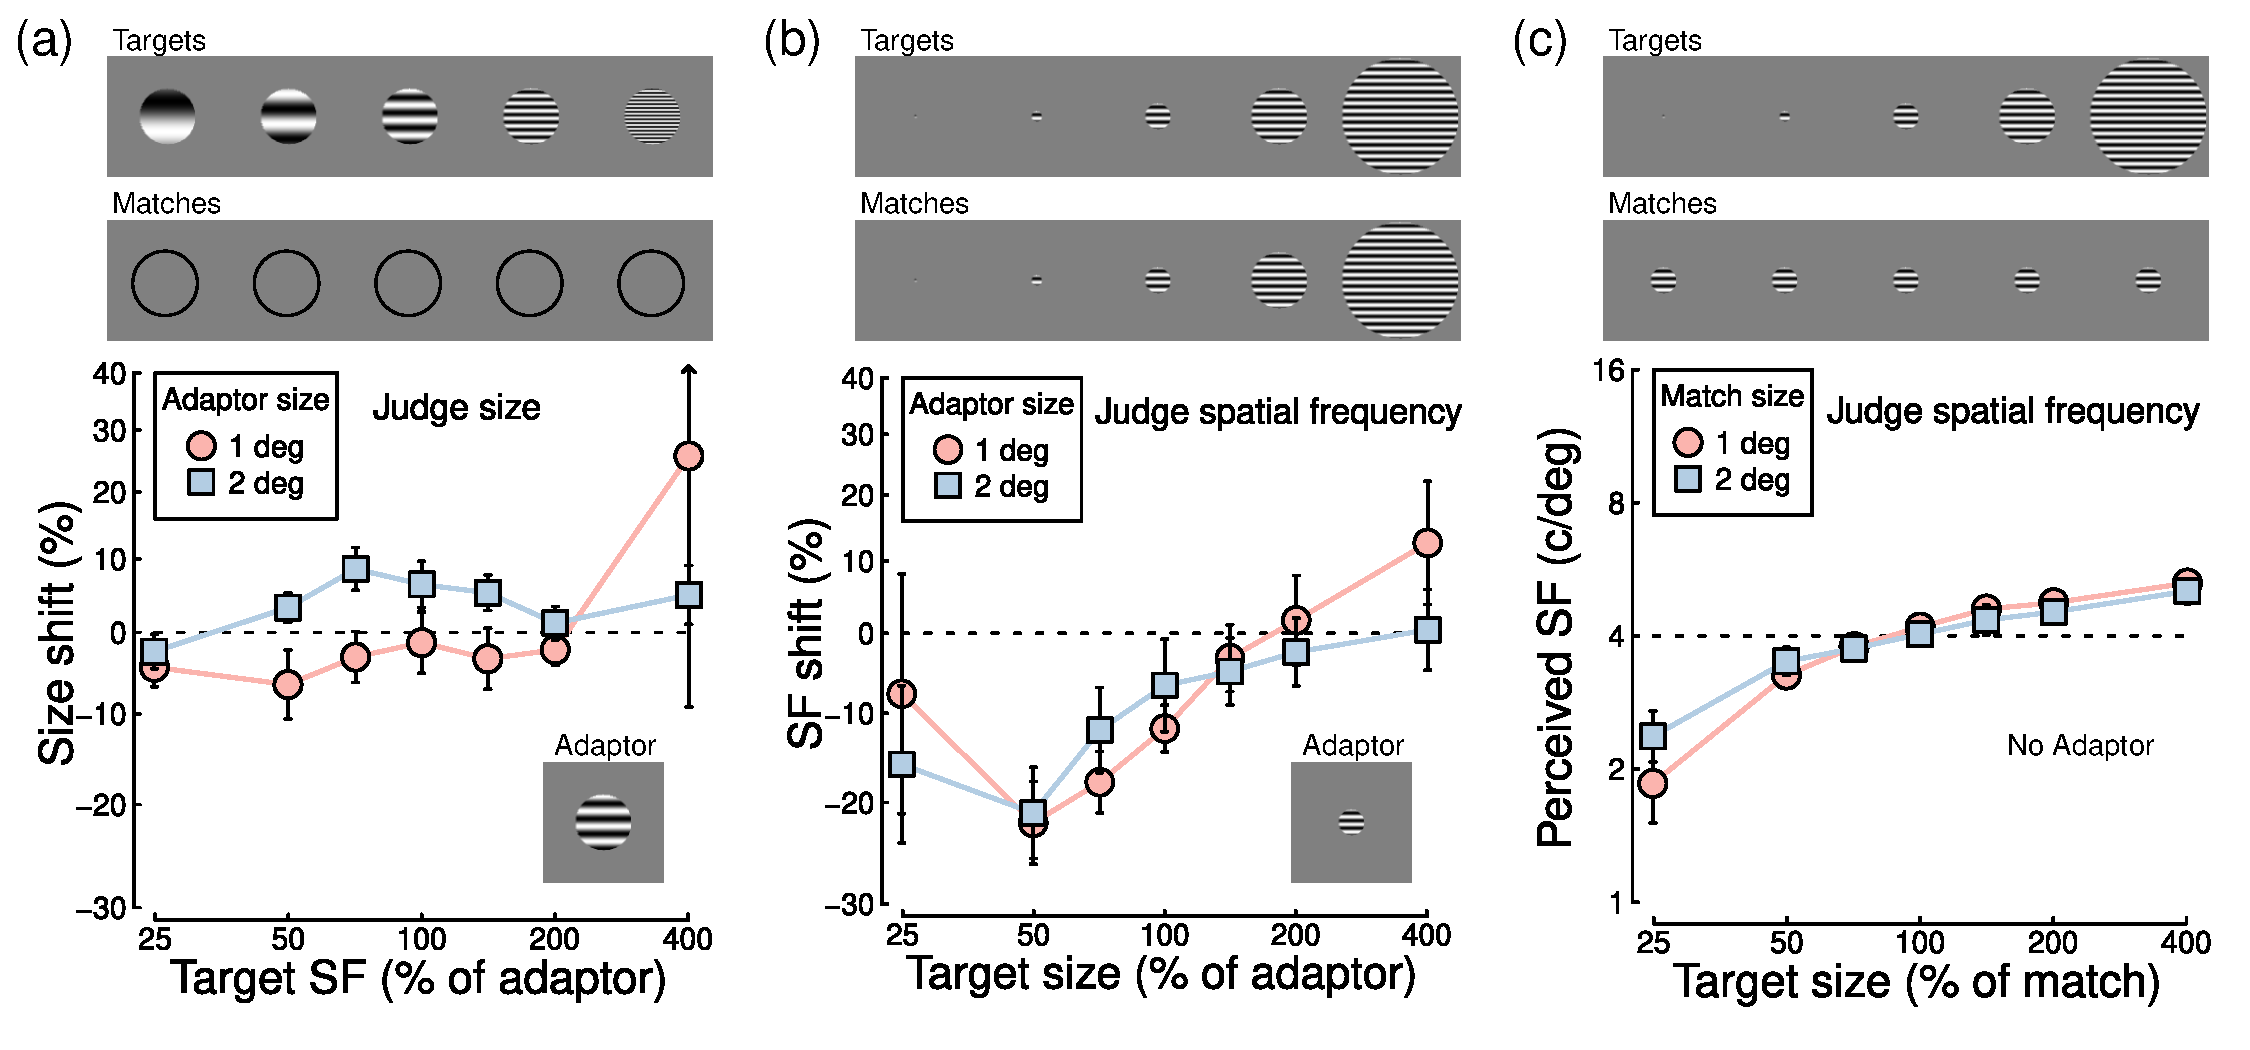
\includegraphics[width=380px]{Figures/Figure4} 

}

\caption{Results from three control experiments ($N$ = 8 participants). Panels (a) and (b) show effects of adaptation. Panel (c) shows the effect of size on perceived spatial frequency. The stimulus icons (top row) depict examples of the target stimuli relating to the x-axes. (All are for the 1 deg adaptor conditions, where the adaptors are shown by the lower right insets. Adaptors and targets had twice the diameters shown for the 2 deg adaptor condition.) (a) Perceived size for targets differing in spatial frequency from the 4c/deg adaptor but of the same physical size as the adaptor (see symbol shapes). The matching stimulus was a ring (second row of icons). (b) Perceived spatial frequency for targets differing in size from the adaptor but with the same physical spatial frequency (4 c/deg) as the adaptor. The matching stimulus was a patch of grating which was the same physical size as the target. Panels (a) and (b) show results relative to baseline measures where there was no adaptation. (c) The results of a control experiment in which the spatial frequencies of various sized targets were compared to matching stimuli of fixed size (see symbol shapes) and spatial frequency of 4c/deg (dashed line). There was no adaptor in this experiment. The difference between this experiment and the baseline condition for (b) is that in (c), the size of the matching stimulus was fixed, whereas in (b) it was the same as the target. Error bars show ±1SE across participants ($N$=8).}\label{fig:figure4}
\end{figure}

\begin{figure}

{\centering 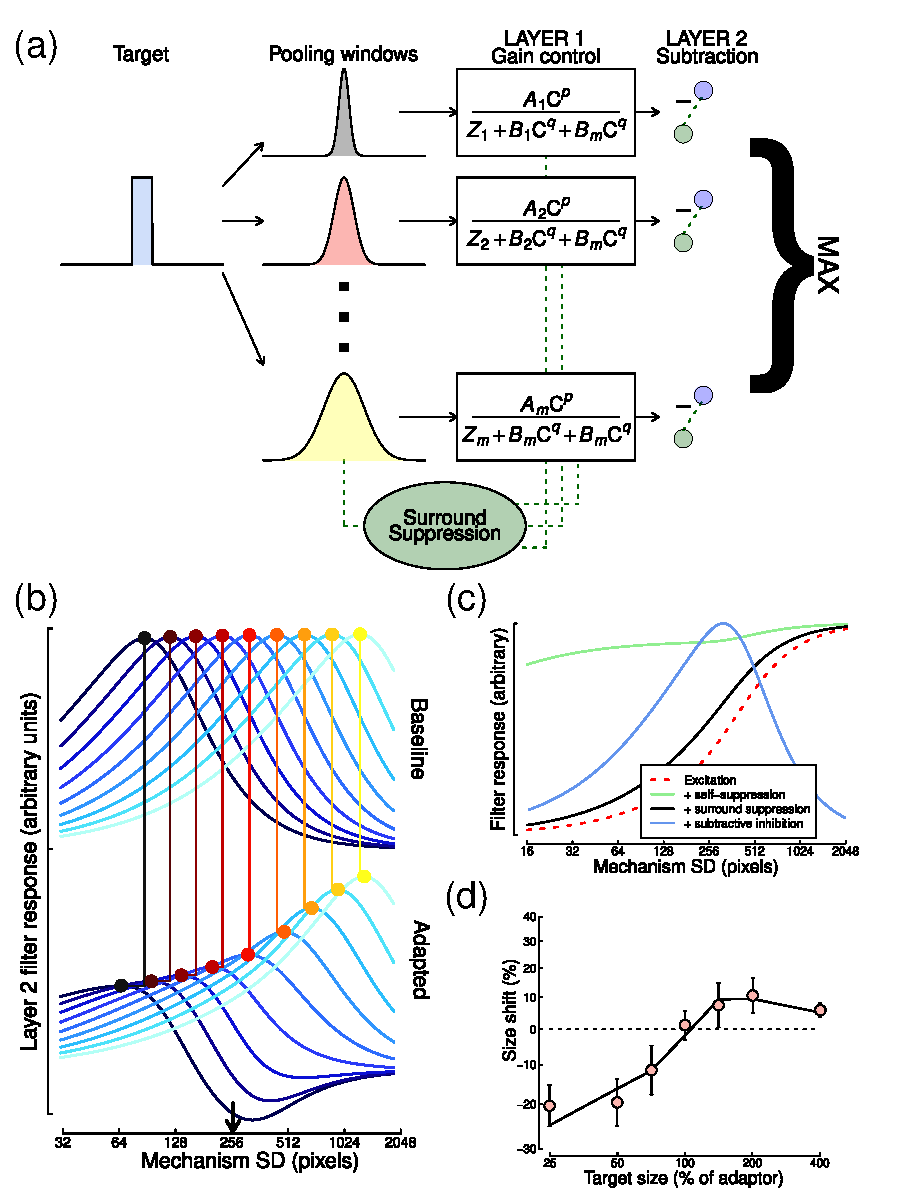
\includegraphics[width=0.7\linewidth]{Figures/Figure5} 

}

\caption{Overview of the computational model. Panel (a) is a schematic of the model. The contrast envelope ($C$) of a stimulus (blue shading) is multiplied by a bank of contrast pooling mechanisms of different spatial widths (only 3 are depicted here; the model had 91). Since we are not modelling the spatial frequency aftereffect, we have excluded the bandpass spatial filtering details for simplicity. Thus, the first explicit stage of our model (Layer 1) is what is traditionally described as a second-order pooling stage where outputs of spatially tuned linear filter-elements are summed over space, phase, orientation and spatial frequency. The results of pooling are passed through a nonlinear stage of gain control involving surround suppression from the largest window ($B_m$). Note that in general, the gain control coefficients, $A$ \& $B$, depend on the sizes of both the stimulus and the relevant pooling window as set out formally in the Methods section. The outputs of Layer 1 are then passed to a second layer involving subtractive inhibition between adjacent mechanisms. The size label of the mechanism with the greatest response in Layer 2 (implied by spline interpolation) delivers an estimate of image size. Adaptation increases the value of $Z$ in Layer 1 in proportion to the mechanism’s response to the adaptor. Panel (b) shows the Layer 2 responses for different sized excitatory pooling windows (x-axis) to stimuli of different sizes (curves), before (top) and after (bottom) adaptation to a 256 pixel-wide adaptor (indicated by the black arrow). The coloured dots indicate the peak response for each condition. Panel (c) shows the effects of the various inhibitory stages on the response distributions across Layers 1 (red, green, black) and 2 (blue) for a single 256 pixel-wide stimulus. Panel (d) shows the adaptation aftereffect, expressed as the percentage change in perceived size (derived from the lateral positions of the coloured dots in panel (c) ($N$ = 8 participants)). The curve is the model behaviour, and the symbols are the 1 deg results replotted from Figure 3a.}\label{fig:figure5}
\end{figure}

\hypertarget{computational-modelling}{%
\subsection*{Computational modelling}\label{computational-modelling}}
\addcontentsline{toc}{subsection}{Computational modelling}

To understand the relationship between size adaptation and population coding involving mechanisms with superimposing selectivity for size, we developed a computational model (described more fully in Appendix A). This was guided by earlier work on contrast perception (Meese et al., 2017; Meese and Baker, 2011; e.g. Meese and Summers, 2007), and devised to overcome the difficulties involved with a simple application of the population model for size coding as described earlier (Figure \ref{fig:figure1}).

For simplicity, our spatially one-dimensional model (see Figure \ref{fig:figure5}a) takes stimulus contrast as input over the spatial extent of the stimulus\footnote{Our model here is devised to deal with psychophysical stimuli---patches of luminance grating in a nominal world of otherwise uniform luminance. In this simple case, no stopping rule is needed for the contrast integration process at the stimulus boundary since the absence of stimulus contrast does the job. In the more general case, an additional process of image segmentation would be needed to identify the boundary of the integration process. We pick up on this point in the discussion.} (i.e.~it treats the envelope of the stimulus as a local measure of contrast)\footnote{To a first approximation this simplification is equivalent to a measure of local (receptive field size) RMS contrast at each point across the image which can be derived from the square root of the sum of the squares of a quadrature pair of filter outputs (i.e.~a standard model complex cell). All of our stimuli were uniform patches of grating (albeit of various sizes). Thus, across most of the stimulus, the local RMS contrast is simply the contrast of the stimulus which is uniform across the stimulus region and zero beyond the stimulus region (see footnote 1). By using the stimulus envelope as a proxy for this measure, we are ignoring minor edge effects (contrast blurring) that would be produced by first-order spatial filters had we included a convolution stage in the model.}, regardless of spatial frequency and orientation (Meese and Baker, 2013). (Our model was not intended to explain the spatial frequency aftereffect which has been modelled elsewhere (e.g. Klein et al., 1974), but could be extended to do this with little or no impact on our conclusions here). These spatially distributed contrast responses (Moutsiana et al., 2016) are multiplied by each element in a one-dimensional `size' array of Gaussian pooling mechanisms of various spatial extents (windows) (dashed red curve in Figure \ref{fig:figure5}c), each member of the array being subject to nonlinear gain control. This includes (i) self-suppression to protect the system's image contrast code from the influence of stimulus size above threshold (Meese and Baker, 2011) (green curve in Figure \ref{fig:figure5}c), (ii) a divisive surround suppression term (Cavanaugh et al., 2002; Sengpiel et al., 1998; Webb et al., 2003; Xing and Heeger, 2001), where each mechanism is suppressed by the largest mechanism in the array (black curve in Figure \ref{fig:figure5}c) to provide the initial basis for size coding (Meese and Baker, 2011) and (iii) a saturation constant (\(Z\)) that allows for the benefit of stimulus size at detection threshold (Meese and Summers, 2012). This has the same initial value for each mechanism (Meese, 2004) but is influenced by the mechanism's response to the adaptor (R) and the gain of adaptation (\(\alpha\)) (Foley and Chen, 1997; Meese and Holmes, 2002) such that \(Z_j = 1 + \alpha R_j\), where \emph{j} indexes the array (i.e.~population) of size mechanisms. In general, with no adaptation this model arrangement produces a distribution of activity across the size array (model Layer 1) with the form of a blurred step edge (black curve in Figure \ref{fig:figure5}c). (See Supplementary Figures \ref{fig:figureS3}-\ref{fig:figureS5} and their captions for further discussion of the model development with and without adaptation.)

First-order image contrast (Meese and Baker, 2011) (not our focus here) and stimulus size (Meese and Baker, 2011) are encoded by the height and location of the distribution of activity across Layer 1, respectively. Note that mechanisms with excitatory pooling regions greater than or equal to the size of the stimulus have comparable responses because they receive the same excitatory drives and suppression. This sets our Layer 1 population code apart from many others in visual perception, where the usual bandpass properties of the mechanisms involved (Figure \ref{fig:figure1}a) result in peaked (bell-shaped) distributions (Figure \ref{fig:figure1}b). Instead, the computational task here is to find where the response transition in the Layer 1 array is located (see black curve in Figure \ref{fig:figure5}c). Following the logic of edge-emphasis by lateral inhibition in the retina (Barlow, 1953), Layer 2 of our model takes a copy of the Layer 1 responses and subjects each to subtractive inhibition from its immediate neighbour, approximating first-order differentiation. This results in size-tuning of the population (blue curve in Figure \ref{fig:figure5}c), with perceived size being given by the peak of the spline-interpolated distribution (Marr and Hildreth, 1980) (see points in the upper row of Figure \ref{fig:figure5}b).

Adaptation is implemented by setting the saturation constant (\emph{Z}, see Foley and Chen, 1997; Meese and Holmes, 2002) in the gain control of Layer 1 such that \(Z_j-1\) is proportional to the \emph{j}th mechanism's response to the adaptor (see Appendix A for details.) Adaptation changes the population size-tuning curves, such that the peaks of the tuning curves in Layer 2 shift away from the adapting stimulus (i.e.~smaller sized stimuli produce peaks at smaller mechanism widths, and vice versa), as shown in the lower row of Figure \ref{fig:figure5}b: the peaks (marked by the coloured dots) are repulsed laterally from the location of the adaptor following adaptation. The ratio of adapted to unadapted perceived size is shown in Figure \ref{fig:figure5}d (curve) and produces the same bi-directional size adaptation aftereffect that we observed empirically (symbols). Note that the decreases in size are around twice as large as the increases, and that this asymmetry is present in both model and human behaviour. Further investigation on the second author confirmed that the size reduction effects remained strong for even smaller targets, and that size increase effects returned to baseline for larger targets. This is also predicted by the model (see Supplementary Figure \ref{fig:figureS2}). These unusual effects derive from natural asymmetries in our model's architecture. For example, within the mechanisms of Layer 1, adaptation is more influential for smaller integration windows because with less potential for the summing of signal (in the inhibitory pathway as well as the excitatory pathway) these mechanisms are more labile. This is to say that the impact of an increase in \emph{Z} (see Figure \ref{fig:figure5}a) is greater when the values of A and B (\(A_1 \le A_2 \le A_m\); and \(B_1 \le B_2 \le B_m\)) are small than when they are large, and since \emph{Z} is the parameter that carries desensitisation by adaptation, aftereffects are larger for smaller mechanisms. Similarly, for any given mechanism, as target size becomes smaller than the integration window, the impact of adaptation increases for that mechanism. (See Supplementary Figures \ref{fig:figureS4} and \ref{fig:figureS5} and their captions for further discussion.)

In general, the behaviour of our model derives primarily from its architecture; the black curve in Figure \ref{fig:figure5}d was derived by setting a single adaptation parameter (\(\alpha\)) by eye (see Methods), yet the model describes the key features of our results (i.e.~their bi-directional asymmetries) very well.

Note that the first layer of our model is consistent with our motivating work on area summation of luminance contrast at threshold and above (Meese, 2004; Meese and Baker, 2011; Meese and Summers, 2007), extending it here by pooling over first-order spatial frequency and orientation, the details of which no doubt deserve further investigation. The second, subtractive, layer is a novel extension designed to deliver the retinal image-size code.

\hypertarget{discussion}{%
\section*{Discussion}\label{discussion}}
\addcontentsline{toc}{section}{Discussion}

We have used an adaptation paradigm to provide the first psychophysical evidence for size mechanisms in human vision, and supported this with a computational model. Other studies have also shown distortions of perceived object shape or size, including various size adaptation aftereffects (Altan and Boyaci, 2020; Köhler and Wallach, 1944; Kreutzer et al., 2015; Laycock et al., 2017; Pooresmaeili et al., 2013; Zeng et al., 2017; Zimmermann et al., 2016). However, none of these studies have demonstrated that vision involves neural mechanisms for size coding. For example, where static luminance-defined shapes or contours have been used, perceptual distortions can be attributed to spatial repulsion effects (Ganz, 1964) or to adaptation of low spatial frequency mechanisms (Blakemore and Sutton, 1969). In some cases, the involvement of retinal afterimages might also have been important (see Köhler and Wallach, 1944). In contrast, our own experiments are the first ones designed to investigate the size-mechanism hypothesis directly, ruling out the possibilities above by using (i) a rapid spatially jittering adaptor and (ii) stimuli that are narrowband in spatial frequency. This approach decouples object size from (i) retinal contour location and (ii) carrier (or dominant object) spatial frequency. We have also placed our results in a computational context developed here by building in a natural way on known cortical physiology and a large body of previous psychophysical work on early vision. We know of no other image-driven model of size perception that has done this. Our model accommodated our hypothesised bi-directional adaptation aftereffects for size, and in this respect the work here delivers a successful test of our proposal about size-coding that emerged from work on image contrast (Meese and Baker, 2011). But more than that, two asymmetrical features of our results that we had not anticipated are emergent properties of our model and provide further support for the scheme we have been advocating.

Our work is complemented by several other studies and observations. For example, the perceived aspect ratio of a shape can be distorted by adaptation, appearing narrower or wider when observers were adapted to other shapes (Storrs and Arnold, 2017) or to large grating patterns (Frome et al., 1979). Haptic size adaptation has also been demonstrated using paradigms where participants grasped objects of different sizes (Walker and Shea, 1974). And more generally, strong simultaneous effects on perceived size can also be induced by surrounding elements that are either smaller or larger than a central target, such as in the well-known Ebbinghaus illusion (Ebbinghaus, 1902).

Our focus here has not been on temporal dynamics, but in additional pilot experiments conducted on the second author, we found that the size effect increased monotonically during the first 16 seconds of adaptation but was constant thereafter. Size perception returned to baseline by around 60 seconds after the offset of the adaptor. This rapid attack and long persistence mean that judgements of object size in natural environments might be affected in repetitive tasks such as fruit picking or production line work, for example. There might also be important clinical implications relating to judgements of body size in patients with eating disorders (Challinor et al., 2017).

Our motivation for this work was the prediction that populations of neurons which pool image texture across various regions of the visual field might code for object size (Meese and Baker, 2011). Receptive fields in V1 are too small for this, but neurons with large receptive fields that also exhibit suppression effects are found in extra-striate visual areas such as V4 (Desimone and Schein, 1987; Pollen et al., 2002) and have many of the required properties. Results from fMRI have shown that adaptation can reduce or increase the area of V1 activated by a stimulus (Pooresmaeili et al., 2013) and this might suggest that our own adaptation effects occur at an earlier stage than we suppose. However, the slow time-course of fMRI means that feedback from later stages might also be involved in these imaging results. A recent study applying TMS to lateral occipital cortex (Zeng et al., 2020) found that size judgements were disrupted at an earlier time point than when TMS was applied to early visual cortex, consistent with this feedback hypothesis.

Our modelling shows how mutually inhibitory mechanisms that pool over different regions of the visual field can produce an adaptable population code for size, but several developments are needed before a more comprehensive understanding of perceived object size can emerge. For simplicity, our current model is one dimensional and (quite straightforwardly) would need to be extended to the two spatial dimensions of the retina to have general applicability. More challenging is that our current model has no method for segmenting the background to deliver a stopping rule for contrast integration, this shortfall owing to the simplicity of our psychophysical constraints. However, our work is not undermined by this, and remains valid so long as the segmentation task can be achieved. Everyday observations serve as an existence proof for this, and our finding that size adaptation aftereffects extend across the orientation and spatial frequency of luminance modulations points to the sort of general second-order process that we should expect (see also Richard et al., 2019): one that operates on the envelope of pooled local contrasts (e.g.~the boundary of an object). Furthermore, visual neurons in V2 and V4 (Zhou et al., 2000) are known to have the border ownership properties that might be an important part of this process, the details of which continue to be investigated (Heydt and Zhang, 2018). Finally, our experiments did not distinguish between image size (which depends on viewing distance) and physical object size (which does not), so whether the process identified here comes before or after the processes of depth perception and size constancy remains to be elucidated. We hope that future work in neuroimaging and neurophysiology as well as psychophysics, will help to illuminate these issues.

\hypertarget{appendix-a-a-computational-model-of-size-adaptation}{%
\section*{Appendix A: A computational model of size adaptation}\label{appendix-a-a-computational-model-of-size-adaptation}}
\addcontentsline{toc}{section}{Appendix A: A computational model of size adaptation}

We constructed a computational model to simulate the size adaptation experiments. For simplicity, the model operates along only one spatial dimension with \emph{i} = 1 to \emph{n} pixels (\emph{n} = 8,192). This gives a notional resolution of 256 pixels per degree. This is higher than in the experiments (64 pixels per degree) which were limited by the pixel resolution of the display. The model has a population of \emph{j} = 1 to \emph{m} pooling mechanisms (\emph{m} = 91) defined by Gaussian spatial profiles (\(G_{ij}\)) with standard deviations ranging from 4 to 2048 pixels (or \textasciitilde1 arcmin to 8 degrees) in logarithmic steps of the index j. Model inputs were rectangular functions (see Figure \ref{fig:figure5}a) with unity height and widths between 16 and 4,096 pixels (3.75 arcmin to 16 degrees; 17 sizes in log steps). Half a cycle of a raised cosine function (16 pixels, or 3.75 arcmin wide, consistent with the stimuli in our experiments) was added to each end of these functions to produce profiles with smooth edges. These inputs describe the contrast envelope of our stimuli across space which, to a first approximation, is equivalent to the output of an array of standard model complex cells. (Recall that stimulus and adaptor contrasts were fixed and identical in our experiments.) Stimulus response was calculated by multiplying model inputs by each pooling mechanism, and their products were passed through a nonlinear gain control equation (Layer 1), given by:

\begin{equation}
  L1_j = \frac{\Sigma_{i=1:n}(G_{ij} \times C_i)^p}{Z_j + \Sigma_{i=1:n}(G_{ij} \times C_i)^q + \Sigma_{i=1:n}(G_{im} \times C_i)^q}
\end{equation}

where \(C_i\) is the model input (the contrast envelope) at each pixel location (\emph{i}). Note that the contrast terms are exponentiated before summation, as required by previous work (Baker et al., 2013). The exponents \emph{p} and \emph{q} were fixed at 2.4 and 2 respectively, also based on previous work (Legge and Foley, 1980; Meese and Summers, 2012; Meese and Summers, 2007). \(Z_j\) is a saturation constant with a value of 1 in the absence of adaptation (described further below). The term that includes \(G_{im}\) represents surround suppression from the largest mechanism in the population (indexed by \emph{m}). The \(\Sigma\) symbol denotes summation across space (\emph{i} = 1:\emph{n}). All stimuli and pooling mechanisms were centred in the middle of the spatial array (of size \emph{n}).

There is a special case of our gain control model worthy of consideration. This is when the target stimulus is a uniform contrast signal, as in our experiments here. In this case, and by ignoring the minor complication of the small skirts of our stimuli, Equation 1 simplifies to the following:

\begin{equation}
  \widehat{L1_j} \approx \frac{A_{j} C^{p}} {Z_{j} + B_{j}C^{q} + B_{m}C^{q}}
\end{equation}

where,

\begin{equation}
  A_{j} = S_{j} \Sigma_{i = 1:n} G_{ij}^{p}
\end{equation}

and

\begin{equation}
  B_{j} = S_{j} \Sigma_{i = 1:n} G_{ij}^{q}
\end{equation}

and where \(S_j\) is either the size of the \emph{j}-th mechanism (\emph{j} = 1:\emph{m}) or the size of the stimulus (both in units of \emph{i}), whichever is smaller. Equation 2 is used in Figure \ref{fig:figure5}a to facilitate interpretation of our Layer 1 architecture, but our formal modelling used the more general Equation 1.

Layer 2 of the model involves subtractive inhibition between neighbouring mechanisms:

\begin{equation}
  L2_{j} = L1_{j} - L1_{j-1}.
\end{equation}

The model was presented with stimuli of various sizes, and the size of each stimulus was estimated by fitting a spline to the population response and finding the maximum (Figure \ref{fig:figure5}b). We obtained equivalent results using a maximum likelihood readout rule (Jazayeri and Movshon, 2006), but this did not improve the analysis and was omitted for simplicity. To model the influence of adaptation, we set the saturation constant such that \(Z_j = 1 + \alpha R_j\), where \(\alpha\) is a free parameter that determines the weight of adaptation, consistent with previous work (Foley and Chen, 1997; Meese and Holmes, 2002), and \(R_j\) is the normalized mechanism response of the \emph{j}-th mechanism to the adaptor. We scaled the values of vector \emph{R} between 0 and 1 by dividing by the most responsive mechanism. (Note that \emph{R} = 0 in the absence of adaptation). We set \(\alpha\) = 360 by eye (for all mechanisms) to give an adaptation effect consistent with our empirical results. (Note that \(\alpha\) is the only free parameter in the model.) Model estimates of stimulus size were then recalculated using the adapted values of \(Z_j\). We define the adaptation aftereffect as the ratio of perceived sizes with and without adaptation, expressed as percentage change (see Figure \ref{fig:figure5}d). We found that key model behaviours derived from the model architecture and were not critically dependent on precise parameter values. We also anticipate that a more elaborate two-dimensional version of the model with traditional bandpass front-end filters would behave similarly for the experiments here.

\hypertarget{acknowledgments}{%
\section*{Acknowledgments}\label{acknowledgments}}
\addcontentsline{toc}{section}{Acknowledgments}

We thank our participants for their hard work collecting data across many sessions during 2011. This work was supported by an EPSRC project grant (EP/H000038/1) awarded to Tim S. Meese and Mark A. Georgeson.

\hypertarget{references}{%
\section*{References}\label{references}}
\addcontentsline{toc}{section}{References}

\hypertarget{refs}{}
\begin{CSLReferences}{1}{0}
\leavevmode\vadjust pre{\hypertarget{ref-Altan2020}{}}%
Altan E, Boyaci H. 2020. Size aftereffect is non-local. \emph{Vision Research} \textbf{176}:40--47. doi:\href{https://doi.org/10.1016/j.visres.2020.07.006}{10.1016/j.visres.2020.07.006}

\leavevmode\vadjust pre{\hypertarget{ref-Arnold1982}{}}%
Arnold KD, Winer GA, Wickens DD. 1982. Veridical and nonveridical interpretations to perceived temperature differences by children and adults. \emph{Bulletin of the Psychonomic Society} \textbf{20}:237--238. doi:\href{https://doi.org/10.3758/BF03334826}{10.3758/BF03334826}

\leavevmode\vadjust pre{\hypertarget{ref-Baker2012}{}}%
Baker DH, Meese TS. 2012. Size adaptation effects are independent of spatial frequency aftereffects. \emph{Perception} \textbf{41(S)}:33.

\leavevmode\vadjust pre{\hypertarget{ref-Baker2013}{}}%
Baker DH, Meese TS, Georgeson MA. 2013. Paradoxical psychometric functions ({``swan functions''}) are explained by dilution masking in four stimulus dimensions. \emph{i-Perception} \textbf{4}:17--35. doi:\href{https://doi.org/10.1068/i0552}{10.1068/i0552}

\leavevmode\vadjust pre{\hypertarget{ref-Baldwin2015}{}}%
Baldwin AS, Meese TS. 2015. Fourth-root summation of contrast over area: No end in sight when spatially inhomogeneous sensitivity is compensated by a witch's hat. \emph{Journal of Vision} \textbf{15}:4. doi:\href{https://doi.org/10.1167/15.15.4}{10.1167/15.15.4}

\leavevmode\vadjust pre{\hypertarget{ref-Barlow1953}{}}%
Barlow HB. 1953. Summation and inhibition in the frog's retina. \emph{The Journal of Physiology} \textbf{119}:69--88. doi:\href{https://doi.org/10.1113/jphysiol.1953.sp004829}{10.1113/jphysiol.1953.sp004829}

\leavevmode\vadjust pre{\hypertarget{ref-Blakemore1971b}{}}%
Blakemore C, Julesz B. 1971. Stereoscopic depth aftereffect produced without monocular cues. \emph{Science} \textbf{171}:286--288. doi:\href{https://doi.org/10.1126/science.171.3968.286}{10.1126/science.171.3968.286}

\leavevmode\vadjust pre{\hypertarget{ref-Blakemore1971}{}}%
Blakemore C, Nachmias J. 1971. The orientation specificity of two visual after-effects. \emph{The Journal of Physiology} \textbf{213}:157--174. doi:\href{https://doi.org/10.1113/jphysiol.1971.sp009374}{10.1113/jphysiol.1971.sp009374}

\leavevmode\vadjust pre{\hypertarget{ref-Blakemore1970}{}}%
Blakemore C, Nachmias J, Sutton P. 1970. The perceived spatial frequency shift: Evidence for frequency-selective neurones in the human brain. \emph{The Journal of Physiology} \textbf{210}:727--750. doi:\href{https://doi.org/10.1113/jphysiol.1970.sp009238}{10.1113/jphysiol.1970.sp009238}

\leavevmode\vadjust pre{\hypertarget{ref-Blakemore1969}{}}%
Blakemore C, Sutton P. 1969. Size adaptation: A new aftereffect. \emph{Science} \textbf{166}:245--247. doi:\href{https://doi.org/10.1126/science.166.3902.245}{10.1126/science.166.3902.245}

\leavevmode\vadjust pre{\hypertarget{ref-Cannon1988}{}}%
Cannon MW, Fullenkamp SC. 1988. Perceived contrast and stimulus size: Experiment and simulation. \emph{Vision Research} \textbf{28}:695--709. doi:\href{https://doi.org/10.1016/0042-6989(88)90049-1}{10.1016/0042-6989(88)90049-1}

\leavevmode\vadjust pre{\hypertarget{ref-Cavanaugh2002}{}}%
Cavanaugh JR, Bair W, Movshon JA. 2002. Nature and interaction of signals from the receptive field center and surround in macaque V1 neurons. \emph{Journal of Neurophysiology} \textbf{88}:2530--2546. doi:\href{https://doi.org/10.1152/jn.00692.2001}{10.1152/jn.00692.2001}

\leavevmode\vadjust pre{\hypertarget{ref-Challinor2017}{}}%
Challinor KL, Mond J, Stephen ID, Mitchison D, Stevenson RJ, Hay P, Brooks KR. 2017. Body size and shape misperception and visual adaptation: An overview of an emerging research paradigm. \emph{Journal of International Medical Research} \textbf{45}:2001--2008. doi:\href{https://doi.org/10.1177/0300060517726440}{10.1177/0300060517726440}

\leavevmode\vadjust pre{\hypertarget{ref-Christman1954}{}}%
Christman RJ. 1954. Shifts in pitch as a function of prolonged stimulation with pure tones. \emph{The American Journal of Psychology} \textbf{67}:484. doi:\href{https://doi.org/10.2307/1417939}{10.2307/1417939}

\leavevmode\vadjust pre{\hypertarget{ref-Coltheart1971}{}}%
Coltheart M. 1971. Visual feature-analyzers and aftereffects of tilt and curvature. \emph{Psychological Review} \textbf{78}:114--121. doi:\href{https://doi.org/10.1037/h0030639}{10.1037/h0030639}

\leavevmode\vadjust pre{\hypertarget{ref-Desimone1987}{}}%
Desimone R, Schein SJ. 1987. Visual properties of neurons in area V4 of the macaque: Sensitivity to stimulus form. \emph{Journal of Neurophysiology} \textbf{57}:835--868. doi:\href{https://doi.org/10.1152/jn.1987.57.3.835}{10.1152/jn.1987.57.3.835}

\leavevmode\vadjust pre{\hypertarget{ref-Ebbinghaus1902}{}}%
Ebbinghaus H. 1902. Grundzuge der psychologie. Leipzig: Verlag von Viet \& Co.

\leavevmode\vadjust pre{\hypertarget{ref-Foley1994}{}}%
Foley JM. 1994. Human luminance pattern-vision mechanisms: Masking experiments require a new model. \emph{Journal of the Optical Society of America A, Optics, Image Science, and Vision} \textbf{11}:1710--1719. doi:\href{https://doi.org/10.1364/josaa.11.001710}{10.1364/josaa.11.001710}

\leavevmode\vadjust pre{\hypertarget{ref-Foley1997}{}}%
Foley JM, Chen CC. 1997. Analysis of the effect of pattern adaptation on pattern pedestal effects: A two-process model. \emph{Vision Research} \textbf{37}:2779--2788. doi:\href{https://doi.org/10.1016/s0042-6989(97)00081-3}{10.1016/s0042-6989(97)00081-3}

\leavevmode\vadjust pre{\hypertarget{ref-Frome1979}{}}%
Frome F, Levinson J, Danielson J, Clavadetscher J. 1979. Shifts in perception of size after adaptation to gratings. \emph{Science} \textbf{206}:1327--1329. doi:\href{https://doi.org/10.1126/science.515736}{10.1126/science.515736}

\leavevmode\vadjust pre{\hypertarget{ref-Ganz1964}{}}%
Ganz L. 1964. Lateral inhibition and the location of visual contours. An analysis of figural after-effects. \emph{Vision Research} \textbf{4}:465--481. doi:\href{https://doi.org/10.1016/0042-6989(64)90053-7}{10.1016/0042-6989(64)90053-7}

\leavevmode\vadjust pre{\hypertarget{ref-Georgeson1980}{}}%
Georgeson MA. 1980. Spatial frequency analysis in early visual processing. \emph{Philosophical Transactions of the Royal Society of London Series B, Biological Sciences} \textbf{290}:11--22. doi:\href{https://doi.org/10.1098/rstb.1980.0079}{10.1098/rstb.1980.0079}

\leavevmode\vadjust pre{\hypertarget{ref-Gibson1937}{}}%
Gibson JJ, Radner M. 1937. Adaptation, after-effect and contrast in the perception of tilted lines. I. Quantitative studies. \emph{Journal of Experimental Psychology} \textbf{20}:453--467. doi:\href{https://doi.org/10.1037/h0059826}{10.1037/h0059826}

\leavevmode\vadjust pre{\hypertarget{ref-Harris2000}{}}%
Harris JP, Wink B. 2000. Invariance of the perceived spatial frequency shift of peripherally viewed gratings with manipulations of contrast, duration, and luminance. \emph{Vision Research} \textbf{40}:931--941. doi:\href{https://doi.org/10.1016/S0042-6989(99)00236-9}{10.1016/S0042-6989(99)00236-9}

\leavevmode\vadjust pre{\hypertarget{ref-Heeley1979}{}}%
Heeley DW. 1979. A perceived spatial frequency shift at orientations orthogonal to adapting gratings. \emph{Vision Research} \textbf{19}:1229--1236. doi:\href{https://doi.org/10.1016/0042-6989(79)90188-3}{10.1016/0042-6989(79)90188-3}

\leavevmode\vadjust pre{\hypertarget{ref-Heron2012}{}}%
Heron J, Aaen-Stockdale C, Hotchkiss J, Roach NW, McGraw PV, Whitaker D. 2012. Duration channels mediate human time perception. \emph{Proceedings of the Royal Society B: Biological Sciences} \textbf{279}:690--698. doi:\href{https://doi.org/10.1098/rspb.2011.1131}{10.1098/rspb.2011.1131}

\leavevmode\vadjust pre{\hypertarget{ref-Heydt2018}{}}%
Heydt R von der, Zhang NR. 2018. Figure and ground: How the visual cortex integrates local cues for global organization. \emph{Journal of Neurophysiology} \textbf{120}:3085--3098. doi:\href{https://doi.org/10.1152/jn.00125.2018}{10.1152/jn.00125.2018}

\leavevmode\vadjust pre{\hypertarget{ref-Jazayeri2006}{}}%
Jazayeri M, Movshon JA. 2006. Optimal representation of sensory information by neural populations. \emph{Nature Neuroscience} \textbf{9}:690--696. doi:\href{https://doi.org/10.1038/nn1691}{10.1038/nn1691}

\leavevmode\vadjust pre{\hypertarget{ref-Klein1974}{}}%
Klein S, Stromeyer CF, Ganz L. 1974. The simultaneous spatial frequency shift: A dissociation between the detection and perception of gratings. \emph{Vision Research} \textbf{14}:1421--1432. doi:\href{https://doi.org/10.1016/0042-6989(74)90017-0}{10.1016/0042-6989(74)90017-0}

\leavevmode\vadjust pre{\hypertarget{ref-Kohler1944}{}}%
Köhler W, Wallach H. 1944. \href{http://www.jstor.org/stable/985451}{Figural after-effects. An investigation of visual processes}. \emph{Proceedings of the American Philosophical Society} \textbf{88}:269--357.

\leavevmode\vadjust pre{\hypertarget{ref-Kreutzer2015}{}}%
Kreutzer S, Fink GR, Weidner R. 2015. Attention modulates visual size adaptation. \emph{Journal of Vision} \textbf{15}:10. doi:\href{https://doi.org/10.1167/15.15.10}{10.1167/15.15.10}

\leavevmode\vadjust pre{\hypertarget{ref-Lawless1991}{}}%
Lawless HT. 1991. A sequential contrast effect in odor perception. \emph{Bulletin of the Psychonomic Society} \textbf{29}:317--319. doi:\href{https://doi.org/10.3758/BF03333930}{10.3758/BF03333930}

\leavevmode\vadjust pre{\hypertarget{ref-Laycock2017}{}}%
Laycock R, Sherman JA, Sperandio I, Chouinard PA. 2017. Size aftereffects are eliminated when adaptor stimuli are prevented from reaching awareness by continuous flash suppression. \emph{Frontiers in Human Neuroscience} \textbf{11}:479. doi:\href{https://doi.org/10.3389/fnhum.2017.00479}{10.3389/fnhum.2017.00479}

\leavevmode\vadjust pre{\hypertarget{ref-Legge1980}{}}%
Legge GE, Foley JM. 1980. Contrast masking in human vision. \emph{Journal of the Optical Society of America} \textbf{70}:1458--1471.

\leavevmode\vadjust pre{\hypertarget{ref-Marks1994}{}}%
Marks LE. 1994. "Recalibrating" the auditory system: The perception of loudness. \emph{J Exp Psychol Hum Percept Perform} \textbf{20}:382--96. doi:\href{https://doi.org/10.1037//0096-1523.20.2.382}{10.1037//0096-1523.20.2.382}

\leavevmode\vadjust pre{\hypertarget{ref-Marr1980}{}}%
Marr D, Hildreth E. 1980. Theory of edge detection. \emph{Proceedings of the Royal Society of London Series B, Biological Sciences} \textbf{207}:187--217. doi:\href{https://doi.org/10.1098/rspb.1980.0020}{10.1098/rspb.1980.0020}

\leavevmode\vadjust pre{\hypertarget{ref-Mather2008}{}}%
Mather G, Pavan A, Campana G, Casco C. 2008. The motion aftereffect reloaded. \emph{Trends in Cognitive Sciences} \textbf{12}:481--487. doi:\href{https://doi.org/10.1016/j.tics.2008.09.002}{10.1016/j.tics.2008.09.002}

\leavevmode\vadjust pre{\hypertarget{ref-Meese2010}{}}%
Meese TS. 2010. Spatially extensive summation of contrast energy is revealed by contrast detection of micro-pattern textures. \emph{Journal of Vision} \textbf{10}:14. doi:\href{https://doi.org/10.1167/10.8.14}{10.1167/10.8.14}

\leavevmode\vadjust pre{\hypertarget{ref-Meese2004}{}}%
Meese TS. 2004. Area summation and masking. \emph{Journal of Vision} \textbf{4}:8. doi:\href{https://doi.org/10.1167/4.10.8}{10.1167/4.10.8}

\leavevmode\vadjust pre{\hypertarget{ref-Meese2013}{}}%
Meese TS, Baker DH. 2013. A common rule for integration and suppression of luminance contrast across eyes, space, time, and pattern. \emph{i-Perception} \textbf{4}:1--16. doi:\href{https://doi.org/10.1068/i0556}{10.1068/i0556}

\leavevmode\vadjust pre{\hypertarget{ref-Meese2011}{}}%
Meese TS, Baker DH. 2011. Contrast summation across eyes and space is revealed along the entire dipper function by a "swiss cheese" stimulus. \emph{Journal of Vision} \textbf{11}:23--23. doi:\href{https://doi.org/10.1167/11.1.23}{10.1167/11.1.23}

\leavevmode\vadjust pre{\hypertarget{ref-Meese2017}{}}%
Meese TS, Baker DH, Summers RJ. 2017. Perception of global image contrast involves transparent spatial filtering and the integration and suppression of local contrasts (not RMS contrast). \emph{Royal Society Open Science} \textbf{4}:170285. doi:\href{https://doi.org/10.1098/rsos.170285}{10.1098/rsos.170285}

\leavevmode\vadjust pre{\hypertarget{ref-Meese2005}{}}%
Meese TS, Hess RF, Williams CB. 2005. Size matters, but not for everyone: Individual differences for contrast discrimination. \emph{Journal of Vision} \textbf{5}:928--947. doi:\href{https://doi.org/10.1167/5.11.2}{10.1167/5.11.2}

\leavevmode\vadjust pre{\hypertarget{ref-Meese2002}{}}%
Meese TS, Holmes DJ. 2002. Adaptation and gain pool summation: Alternative models and masking data. \emph{Vision Research} \textbf{42}:1113--1125. doi:\href{https://doi.org/10.1016/S0042-6989(01)00291-7}{10.1016/S0042-6989(01)00291-7}

\leavevmode\vadjust pre{\hypertarget{ref-Meese2012}{}}%
Meese TS, Summers RJ. 2012. Theory and data for area summation of contrast with and without uncertainty: Evidence for a noisy energy model. \emph{Journal of Vision} \textbf{12}:9--9. doi:\href{https://doi.org/10.1167/12.11.9}{10.1167/12.11.9}

\leavevmode\vadjust pre{\hypertarget{ref-Meese2009}{}}%
Meese TS, Summers RJ. 2009. Neuronal convergence in early contrast vision: Binocular summation is followed by response nonlinearity and area summation. \emph{Journal of Vision} \textbf{9}:7--7. doi:\href{https://doi.org/10.1167/9.4.7}{10.1167/9.4.7}

\leavevmode\vadjust pre{\hypertarget{ref-Meese2007}{}}%
Meese TS, Summers RJ. 2007. Area summation in human vision at and above detection threshold. \emph{Proceedings of the Royal Society B: Biological Sciences} \textbf{274}:2891--2900. doi:\href{https://doi.org/10.1098/rspb.2007.0957}{10.1098/rspb.2007.0957}

\leavevmode\vadjust pre{\hypertarget{ref-Morgan1990}{}}%
Morgan MJ, Ward RM, Hole GJ. 1990. Evidence for positional coding in hyperacuity. \emph{Journal of the Optical Society of America A} \textbf{7}:297. doi:\href{https://doi.org/10.1364/JOSAA.7.000297}{10.1364/JOSAA.7.000297}

\leavevmode\vadjust pre{\hypertarget{ref-Moutsiana2016}{}}%
Moutsiana C, Haas B de, Papageorgiou A, Dijk JA van, Balraj A, Greenwood JA, Schwarzkopf DS. 2016. Cortical idiosyncrasies predict the perception of object size. \emph{Nature Communications} \textbf{7}:12110. doi:\href{https://doi.org/10.1038/ncomms12110}{10.1038/ncomms12110}

\leavevmode\vadjust pre{\hypertarget{ref-Olejnik2003}{}}%
Olejnik S, Algina J. 2003. Generalized eta and omega squared statistics: Measures of effect size for some common research designs. \emph{Psychological Methods} \textbf{8}:434--447. doi:\href{https://doi.org/10.1037/1082-989X.8.4.434}{10.1037/1082-989X.8.4.434}

\leavevmode\vadjust pre{\hypertarget{ref-Pollen2002}{}}%
Pollen DA, Przybyszewski AW, Rubin MA, Foote W. 2002. Spatial receptive field organization of macaque V4 neurons. \emph{Cerebral Cortex} \textbf{12}:601--616. doi:\href{https://doi.org/10.1093/cercor/12.6.601}{10.1093/cercor/12.6.601}

\leavevmode\vadjust pre{\hypertarget{ref-Pooresmaeili2013}{}}%
Pooresmaeili A, Arrighi R, Biagi L, Morrone MC. 2013. Blood oxygen level-dependent activation of the primary visual cortex predicts size adaptation illusion. \emph{Journal of Neuroscience} \textbf{33}:15999--16008. doi:\href{https://doi.org/10.1523/JNEUROSCI.1770-13.2013}{10.1523/JNEUROSCI.1770-13.2013}

\leavevmode\vadjust pre{\hypertarget{ref-Richard2019}{}}%
Richard B, Hansen BC, Johnson AP, Shafto P. 2019. Spatial summation of broadband contrast. \emph{Journal of Vision} \textbf{19}:16. doi:\href{https://doi.org/10.1167/19.5.16}{10.1167/19.5.16}

\leavevmode\vadjust pre{\hypertarget{ref-Roach2011}{}}%
Roach NW, Heron J, Whitaker D, McGraw PV. 2011. Asynchrony adaptation reveals neural population code for audio-visual timing. \emph{Proceedings of the Royal Society B: Biological Sciences} \textbf{278}:1314--1322. doi:\href{https://doi.org/10.1098/rspb.2010.1737}{10.1098/rspb.2010.1737}

\leavevmode\vadjust pre{\hypertarget{ref-Rouder2012}{}}%
Rouder JN, Morey RD, Speckman PL, Province JM. 2012. Default bayes factors for ANOVA designs. \emph{Journal of Mathematical Psychology} \textbf{56}:356--374. doi:\href{https://doi.org/10.1016/j.jmp.2012.08.001}{10.1016/j.jmp.2012.08.001}

\leavevmode\vadjust pre{\hypertarget{ref-Sengpiel1998}{}}%
Sengpiel F, Baddeley RJ, Freeman TC, Harrad R, Blakemore C. 1998. Different mechanisms underlie three inhibitory phenomena in cat area 17. \emph{Vision Research} \textbf{38}:2067--2080. doi:\href{https://doi.org/10.1016/s0042-6989(97)00413-6}{10.1016/s0042-6989(97)00413-6}

\leavevmode\vadjust pre{\hypertarget{ref-Snowden1998}{}}%
Snowden RJ, Hammett ST. 1998. The effects of surround contrast on contrast thresholds, perceived contrast and contrast discrimination. \emph{Vision Research} \textbf{38}:1935--1945. doi:\href{https://doi.org/10.1016/s0042-6989(97)00379-9}{10.1016/s0042-6989(97)00379-9}

\leavevmode\vadjust pre{\hypertarget{ref-Storrs2017}{}}%
Storrs KR, Arnold DH. 2017. Shape adaptation exaggerates shape differences. \emph{Journal of Experimental Psychology: Human Perception and Performance} \textbf{43}:181--191. doi:\href{https://doi.org/10.1037/xhp0000292}{10.1037/xhp0000292}

\leavevmode\vadjust pre{\hypertarget{ref-Sutherland1961}{}}%
Sutherland NS. 1961. Figural after-effects and apparent size. \emph{Quarterly Journal of Experimental Psychology} \textbf{13}:222--228. doi:\href{https://doi.org/10.1080/17470216108416498}{10.1080/17470216108416498}

\leavevmode\vadjust pre{\hypertarget{ref-Tsai2003}{}}%
Tsai JJ, Victor JD. 2003. Reading a population code: A multi-scale neural model for representing binocular disparity. \emph{Vision Research} \textbf{43}:445--466. doi:\href{https://doi.org/10.1016/s0042-6989(02)00510-2}{10.1016/s0042-6989(02)00510-2}

\leavevmode\vadjust pre{\hypertarget{ref-Walker1981}{}}%
Walker JT, Irion AL, Gordon DG. 1981. Simple and contingent aftereffects of perceived duration in vision and audition. \emph{Perception \& Psychophysics} \textbf{29}:475--486. doi:\href{https://doi.org/10.3758/BF03207361}{10.3758/BF03207361}

\leavevmode\vadjust pre{\hypertarget{ref-Walker1974}{}}%
Walker JT, Shea KS. 1974. A tactual size aftereffect contingent on hand position. \emph{Journal of Experimental Psychology} \textbf{103}:668--674. doi:\href{https://doi.org/10.1037/h0037136}{10.1037/h0037136}

\leavevmode\vadjust pre{\hypertarget{ref-Webb2003}{}}%
Webb BS, Tinsley CJ, Barraclough NE, Parker A, Derrington AM. 2003. Gain control from beyond the classical receptive field in primate primary visual cortex. \emph{Visual Neuroscience} \textbf{20}:221--230. doi:\href{https://doi.org/10.1017/s0952523803203011}{10.1017/s0952523803203011}

\leavevmode\vadjust pre{\hypertarget{ref-Webster2008}{}}%
Webster MA, Leonard D. 2008. Adaptation and perceptual norms in color vision. \emph{Journal of the Optical Society of America A} \textbf{25}:2817. doi:\href{https://doi.org/10.1364/JOSAA.25.002817}{10.1364/JOSAA.25.002817}

\leavevmode\vadjust pre{\hypertarget{ref-Xing2001}{}}%
Xing J, Heeger DJ. 2001. Measurement and modeling of center-surround suppression and enhancement. \emph{Vision Research} \textbf{41}:571--583. doi:\href{https://doi.org/10.1016/s0042-6989(00)00270-4}{10.1016/s0042-6989(00)00270-4}

\leavevmode\vadjust pre{\hypertarget{ref-Zeng2020}{}}%
Zeng H, Fink GR, Weidner R. 2020. Visual size processing in early visual cortex follows lateral occipital cortex involvement. \emph{The Journal of Neuroscience} \textbf{40}:4410--4417. doi:\href{https://doi.org/10.1523/JNEUROSCI.2437-19.2020}{10.1523/JNEUROSCI.2437-19.2020}

\leavevmode\vadjust pre{\hypertarget{ref-Zeng2017}{}}%
Zeng H, Kreutzer S, Fink GR, Weidner R. 2017. The source of visual size adaptation. \emph{Journal of Vision} \textbf{17}:8. doi:\href{https://doi.org/10.1167/17.14.8}{10.1167/17.14.8}

\leavevmode\vadjust pre{\hypertarget{ref-Zhou2000}{}}%
Zhou H, Friedman HS, Heydt R von der. 2000. Coding of border ownership in monkey visual cortex. \emph{The Journal of Neuroscience: The Official Journal of the Society for Neuroscience} \textbf{20}:6594--6611. doi:\href{https://doi.org/10.1523/JNEUROSCI.20-17-06594.2000}{10.1523/JNEUROSCI.20-17-06594.2000}

\leavevmode\vadjust pre{\hypertarget{ref-Zimmermann2016}{}}%
Zimmermann E, Morrone MC, Burr D. 2016. Adaptation to size affects saccades with long but not short latencies. \emph{Journal of Vision} \textbf{16}:2. doi:\href{https://doi.org/10.1167/16.7.2}{10.1167/16.7.2}

\end{CSLReferences}

\hypertarget{supplementary-information}{%
\section*{Supplementary information}\label{supplementary-information}}
\addcontentsline{toc}{section}{Supplementary information}

\setcounter{table}{0}  \renewcommand{\thetable}{S\arabic{table}} \setcounter{figure}{0} \renewcommand{\thefigure}{S\arabic{figure}}

\begin{figure}

{\centering 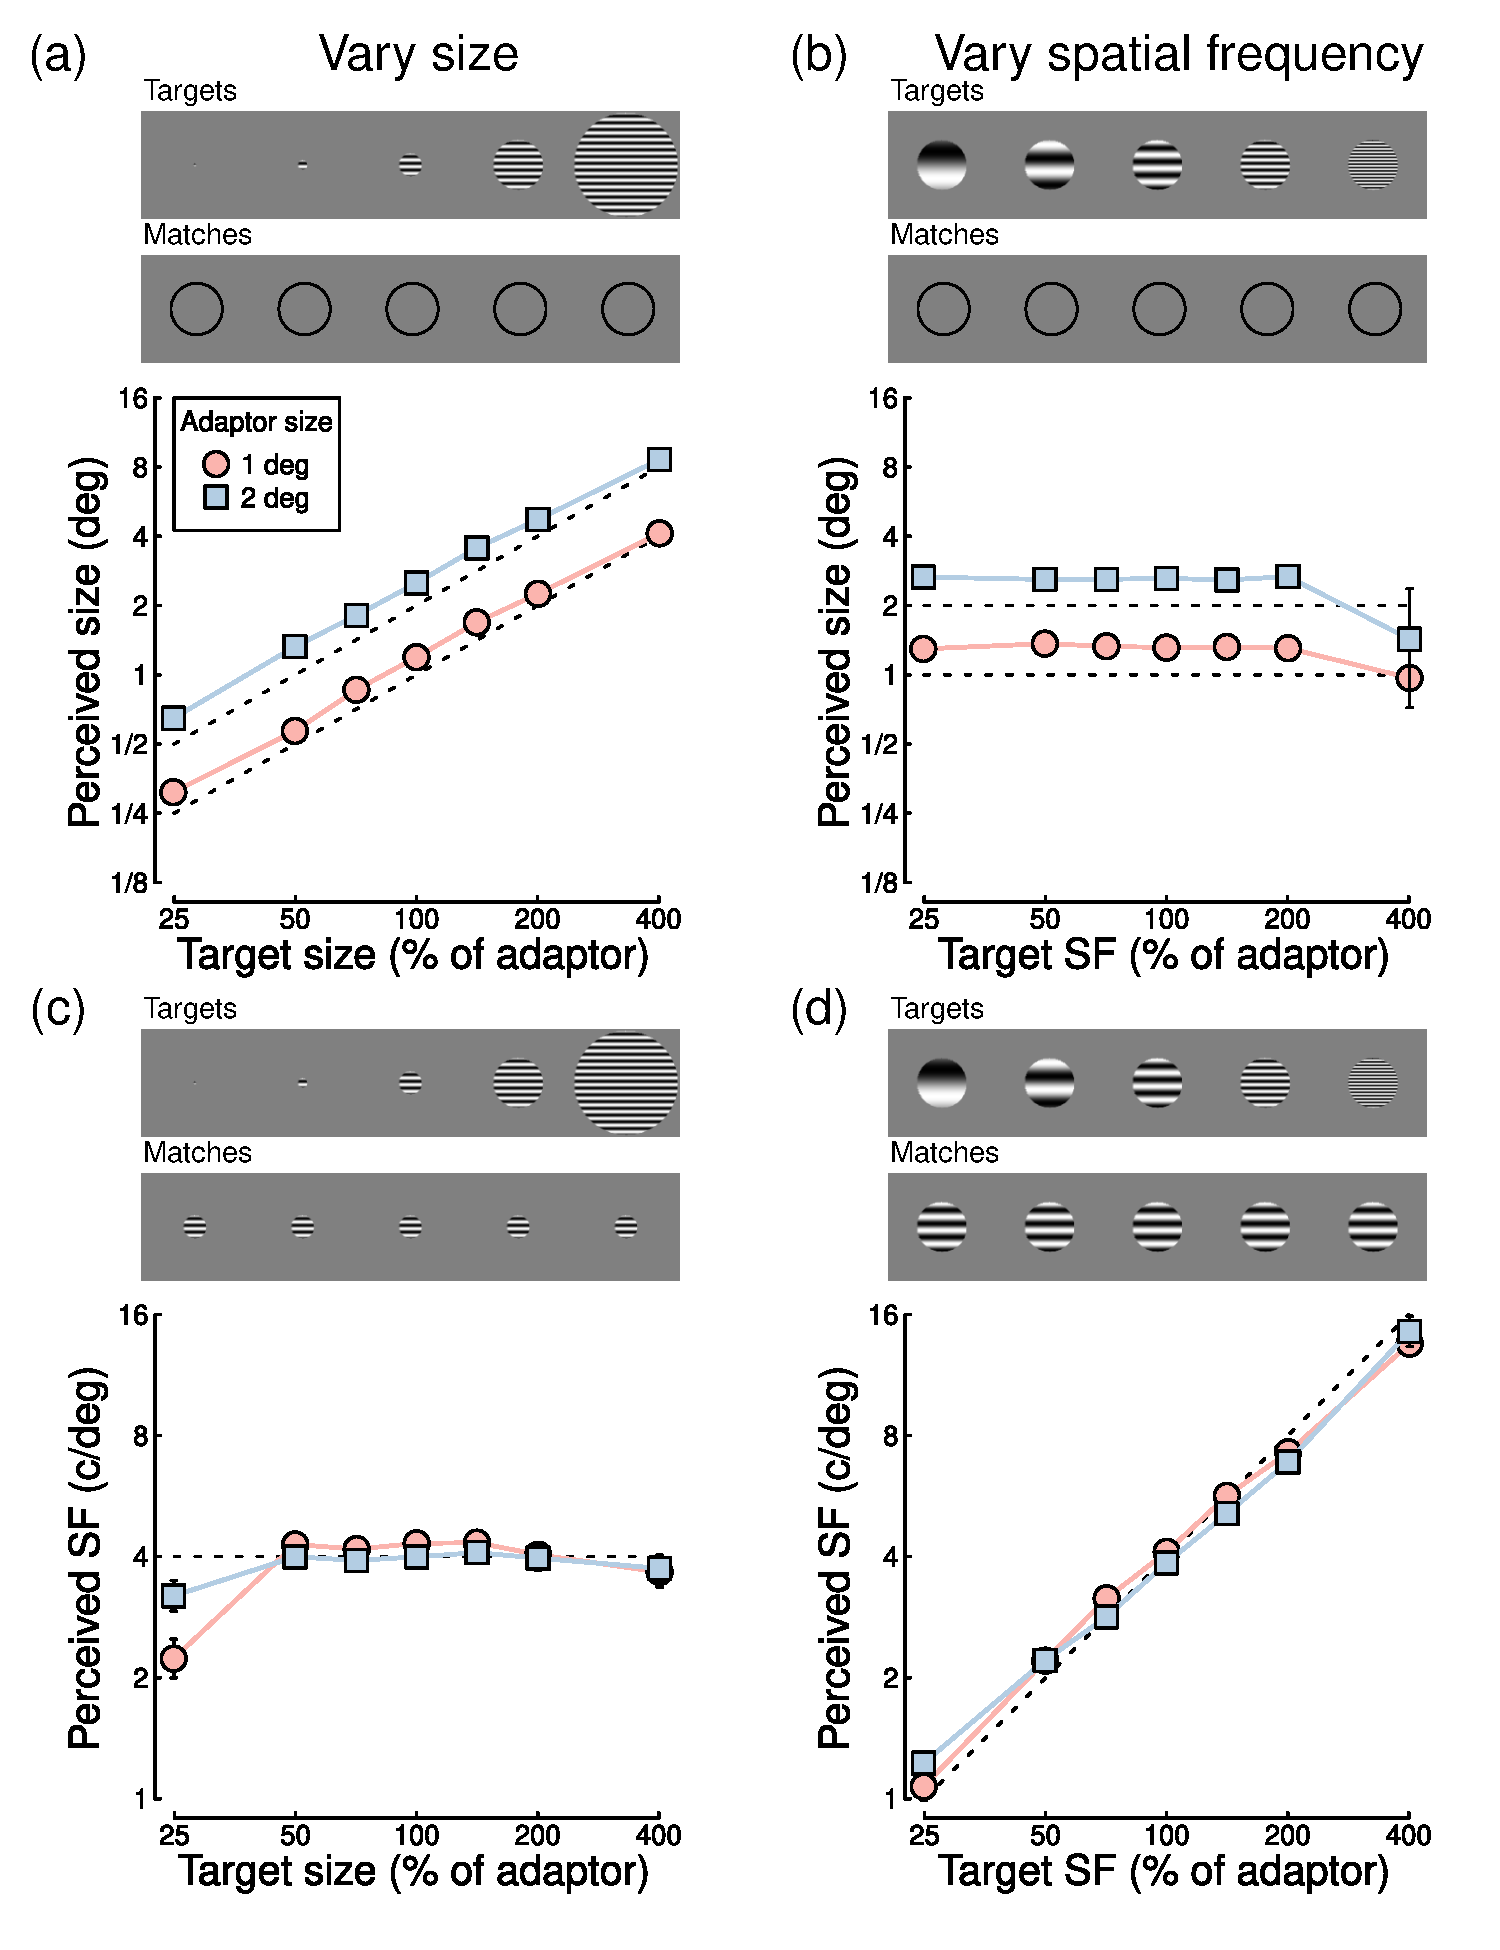
\includegraphics[width=0.8\linewidth]{Figures/FigureS1} 

}

\caption{Baseline settings for perceived size (top) and perceived spatial frequency (bottom) (N = 8 participants). The stimuli were targets that varied in size (left) or in spatial frequency (right). Dashed lines in each panel show the expectation for veridical matches. In general, perceived size was slightly overestimated, most likely a consequence of the raised cosine envelope used to window the grating stimuli which added to the overall diameter. The high variance in the perceived sizes of the highest spatial frequency stimuli (far right points in panel b) is probably because these stimuli were close to detection threshold. Similarly, the spatial frequency was difficult to judge for the smallest targets (far left points in panel c) and was underestimated overall. However, the matches for the baseline conditions from the main experiments were very close to veridical (panels a, d). Error bars indicate ±1SE across participants (N=8), and in most cases are smaller than the symbols.}\label{fig:figureS1}
\end{figure}

\begin{figure}
\centering
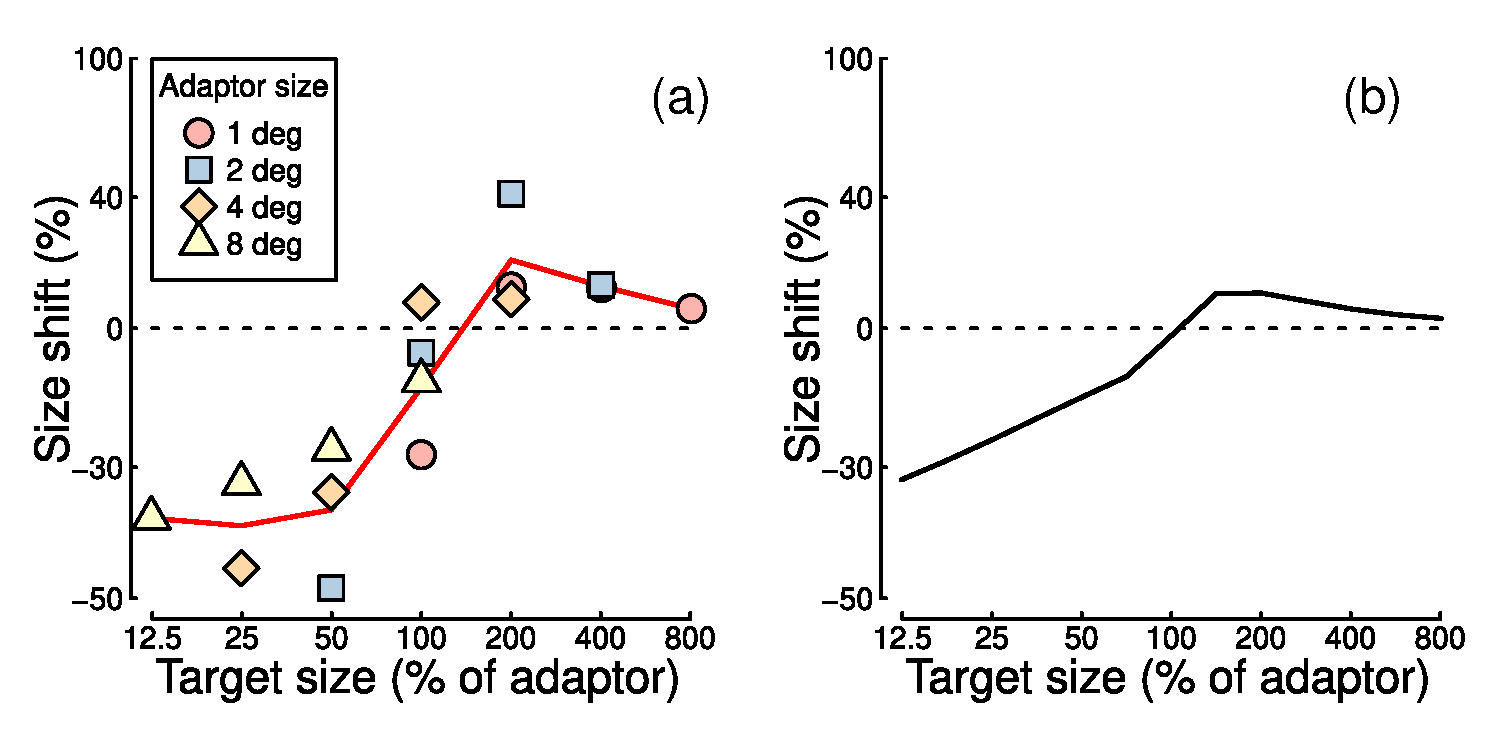
\includegraphics{Figures/FigureS2.pdf}
\caption{\label{fig:figureS2}Results for the second author (a) and model predictions (b) across a wider range of relative target/adaptor sizes than was used in the main experiment (N = 1 participant). The conditions involved factorial combination of four target and adaptor sizes (see legend in panel (a)), and the red curve shows their average. Across this extended range the results confirm our earlier observations: the size reduction aftereffect (left of the plot) does not return to baseline, whereas the size increase aftereffect (right of the plot) returns to baseline for large targets. As in the main experiment, the size reduction aftereffects are much larger than the size increase aftereffects. The model behaviour in panel (b) predicts these features of the results. The adaptation parameter, \(\alpha\), is unchanged from before.}
\end{figure}

\begin{figure}

{\centering 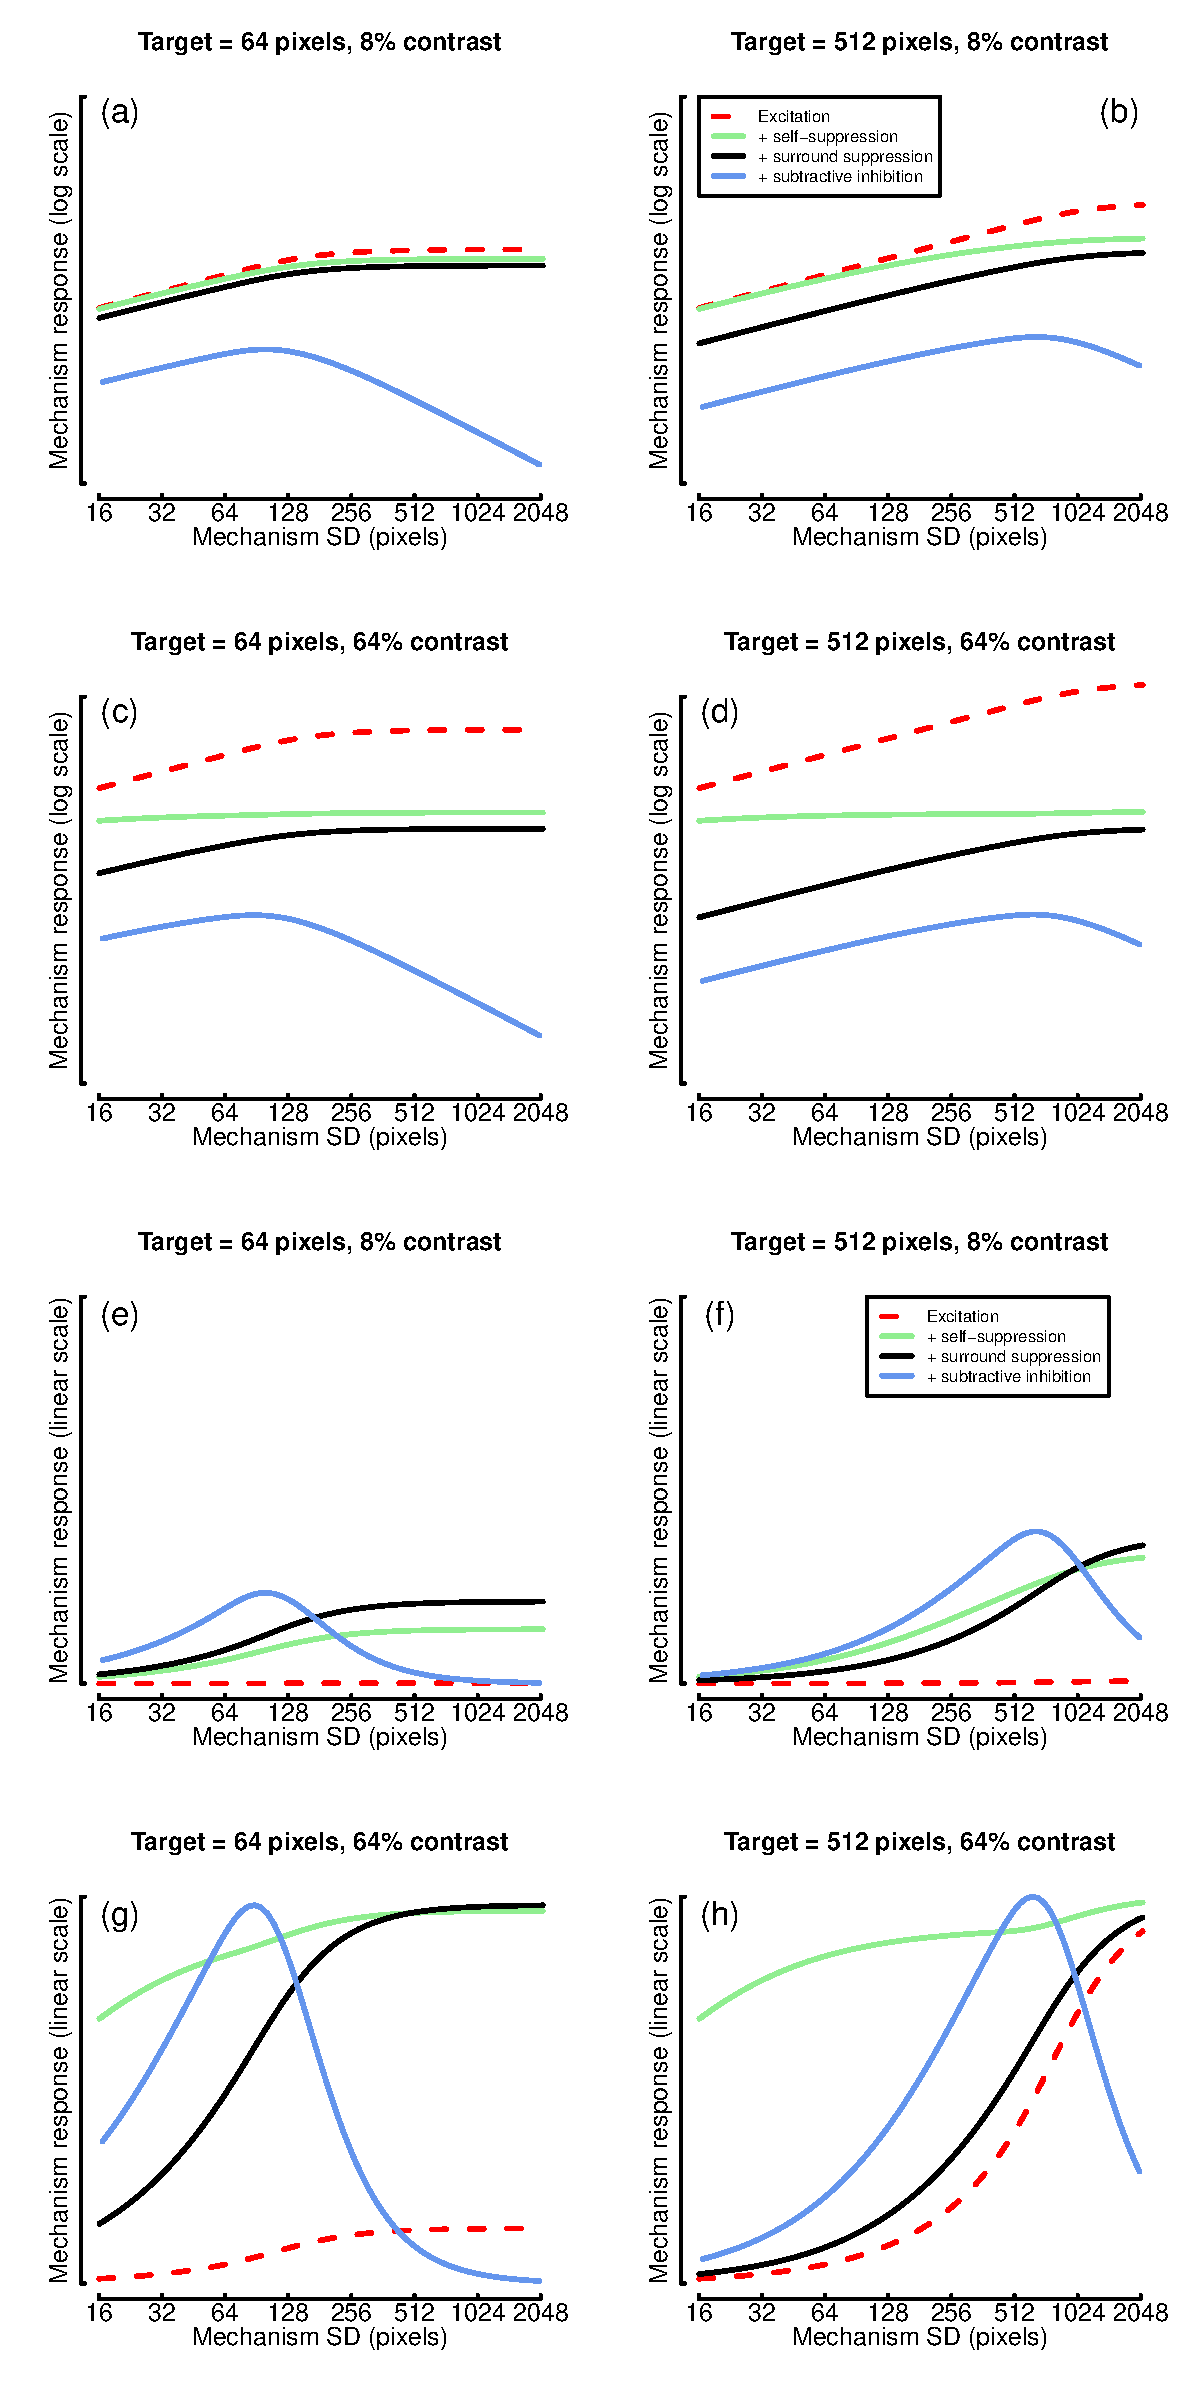
\includegraphics[width=0.5\linewidth]{Figures/FigureS3} 

}

\caption{Mechanism responses as functions of the size (SD) of the integration window. This illustrates population responses with the progressive introduction of various model features (see legend). Panels (a-d) are for double-log axes. The same mechanism responses are shown on linear axes in panels (e-h). The responses are shown for a small (64 pixel wide) stimulus in the left column (a, c, e, g) and a larger (512 pixel wide) stimulus in the right column (b, d, f, h). The first (a, b) and third (e, f) rows are for low (8\%) contrast stimuli, and the second (c, d) and fourth (g, h) rows are for high (64\%) contrast stimuli. For the purpose of illustration in panels (e-h), each function is normalised by the greatest response across panels. The dashed red curves (Layer 1) are for a model with no suppression (no gain control), only excitation and exponentiation (p = 2.4) of the contrast responses for a population of different sized spatial integration windows. The right-hand side of the red response function rises with an increase in stimulus contrast and an increase in stimulus size, resulting in response ambiguity. This ambiguity can be removed by implementing gain control by self-suppression (green curves) in Layer 1. This leaves a contrast effect in the model (first row versus second row), but no clear effect of size (e.g. panel c versus d). This problem is fixed by introducing surround suppression (black curves) in Layer 1. With this arrangement, the height of the population response depends on stimulus contrast (consistent with published contrast discrimination results) and the lateral position of the transition of the population response depends on stimulus size. The blue curves derive from the introduction of lateral inhibition in Layer 2. This converts the maximum gradients in the black functions of Layer 1 to peaks in Layer 2 by a discrete approximation to differentiation. The peaks of these curves are located by a max operator.}\label{fig:figureS3}
\end{figure}

\begin{figure}
\centering
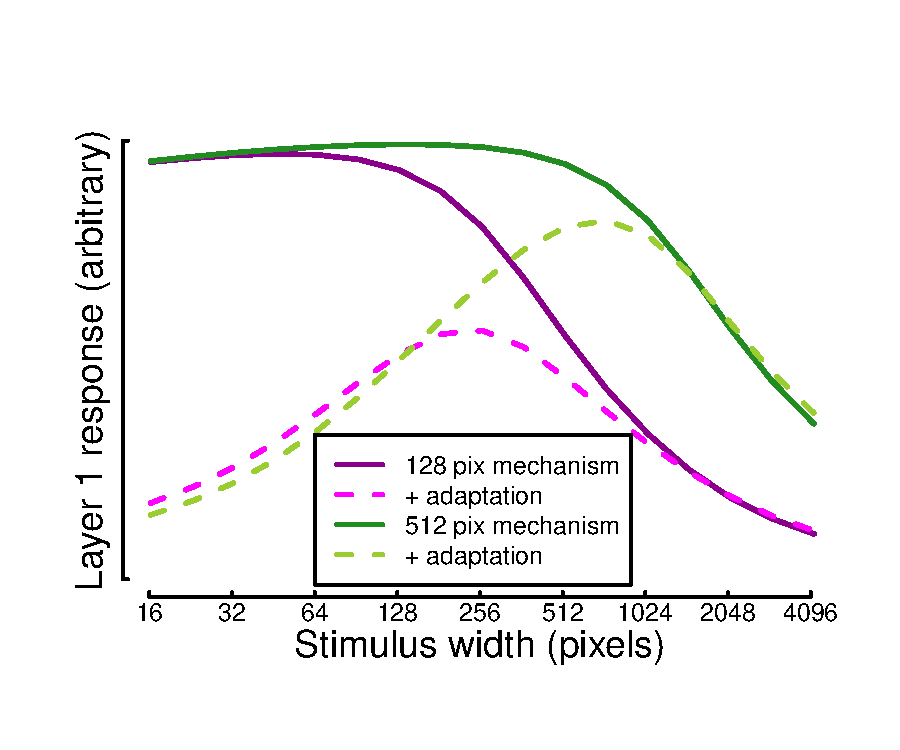
\includegraphics{Figures/FigureS4.pdf}
\caption{\label{fig:figureS4}Responses of two Layer 1 mechanisms in the model as a function of the width/size of a high contrast stimulus. The standard deviations of the integration windows were 128 pixels (pink/purple) and 512 pixels (green). Solid and dashed curves are for the unadapted and adapted states, respectively (for a 256-pixel adaptor). Note that when the stimulus is much smaller than the integration window, increasing stimulus size causes little or no change in response because the benefits of excitatory integration are offset by the effects of suppression in the contrast gain control equation (Equations 1 and 2, and Figure 5a of the main report). However, for stimulus sizes greater than the integration window, responses decrease with stimulus size because of the increasing contribution of surround suppression (the second contrast term on the denominator of Equations 1 and 2, and the Bm term in Figure 5 of the main report) without a concomitant increase in excitation. This arrangement means that the Layer 1 mechanisms can carry a stimulus contrast code unconfound by stimulus size (Meese, 2004; Meese and Summers, 2007; Meese and Baker, 2011, 2013). The situation is different in the adapted state. Here, adaptation is most severe when the test stimulus is smaller than the mechanism's integration window. This is because as the stimulus gets smaller, the A and B terms in Figure 5 of the main report get smaller, and the mechanism is more readily influenced by adaptation which increases the value of Z (see also Equation 1 in the main report). This asymmetry in adaptation contributes to the asymmetries seen in the model's account of our results.}
\end{figure}

\begin{figure}

{\centering 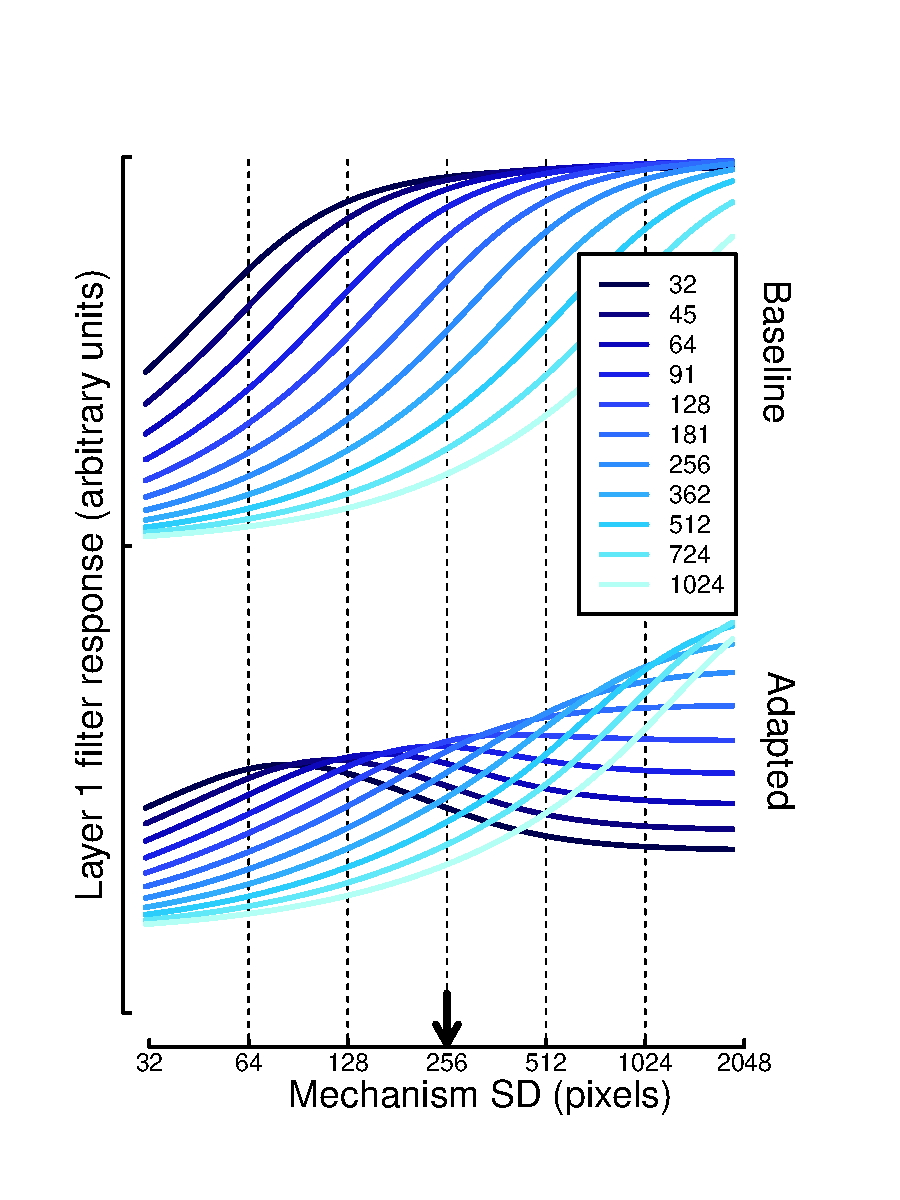
\includegraphics[width=0.8\linewidth]{Figures/FigureS5} 

}

\caption{Responses of Layer 1 mechanisms for different high contrast stimulus width/sizes (shown in the legend in pixel units) as a function of the standard deviation of each mechanism’s integration window. The top panel is for the unadapted/baseline state and the bottom panel is for adaptation to a stimulus with a width/size of 256 pixels (black arrow). This figure is the Layer 1 equivalent of the Layer 2 responses shown in Figure 5b of the main report but extended to smaller stimulus sizes. (The top panel is also the family of curves for which a single instance is shown in Figure 5c of the main report.) At baseline, the population of Layer 1 responses provides a code for image contrast (plateau height) and stimulus size (given by the mechanism’s size label at the transition point in the response distribution and picked off by the differentiation process in Layer 2). The aftereffects of adaptation on the population of Layer 1 responses is asymmetric. This is because the impact of adaptation depends on (i) the mechanism’s sensitivity to the adaptor (top panel), which is asymmetric to the right, but also (ii) the effect of the adaptation term (Z in Figure 5a and Equation 1 of the main report) on the overall mechanism response. This effect increases with a decrease in the integration of signal contrast and is asymmetric to the left. These two asymmetries are not balanced in their influences on the adapted Layer 1 network which is shown by the asymmetry in the bottom panel of the figure. This imbalance contributes to the asymmetries seen in the model’s account of our results.}\label{fig:figureS5}
\end{figure}

\hypertarget{supplementary-movies}{%
\subsection*{Supplementary Movies}\label{supplementary-movies}}
\addcontentsline{toc}{subsection}{Supplementary Movies}

\textbf{Movie S1.} Demonstration of size adaptation with horizontal adaptors and targets. To facilitate a large effect, the viewer should fixate the central cross throughout. The adaptors will jitter on either size of the display. After a brief blank interval, two identical gratings are shown, but they will look different in size following adaptation. Note that the demonstration does not correspond to the stimulus arrangement in the experiment, where a single adaptor was presented to one side only of the display.

\textbf{Movie S2.} As for Movie S1, except that the adaptors have the same size and different spatial frequencies. The aftereffect is a change in the perceived spatial frequency of the carrier but with no change in perceived size.

\textbf{Movie S3.} As for Movie S1, except that the adaptors and targets have orthogonal orientations. The size-aftereffect is seen nonetheless.

\textbf{Movie S4.} As for Movie S1, except that the grating textures are replaced by uniform luminance.

\textbf{Movie S5.} As for Movie S1, except that the target grating is replaced by a face image.

\end{document}
